% TODO: Update this for proper formatting:
%\documentclass[12pt,times]{article}
\documentclass[12pt]{article} % \usepackage{times}
%\usepackage[a4paper, showframe, tmargin=25mm, lmargin=25mm, rmargin=25mm, bmargin=20mm]{geometry}
\usepackage[a4paper, tmargin=25mm, lmargin=20mm, rmargin=20mm, bmargin=20mm]{geometry}
\usepackage{amsmath,amssymb,amsthm}
\usepackage{color}
\usepackage{hyperref}
\usepackage{graphicx}
\usepackage{stmaryrd}
\usepackage{listings}
\usepackage{color}
\usepackage{wrapfig}
\usepackage{url}
\usepackage{fancyvrb}
\usepackage{placeins}
\usepackage{bold-extra}
\usepackage[nounderscore]{syntax}
\usepackage{mathtools}
\usepackage{caption}
\usepackage{float}

%\usepackage{fancyhdr}
%\pagestyle{fancy}
%\rhead{Version: \GUIDEVERSION} 
%\lhead{\GUIDETITLE}
%\cfoot{}
%\thispagestyle{fancy}
% \thispagestyle{headings}


\makeatletter
\renewcommand{\maketitle}{\bgroup\setlength{\parindent}{0pt}
  \thispagestyle{empty}
  \begin{flushleft}
    \textbf{\@title}

    \vspace{3cm}
    
    \@author
    
    \begin{center}
      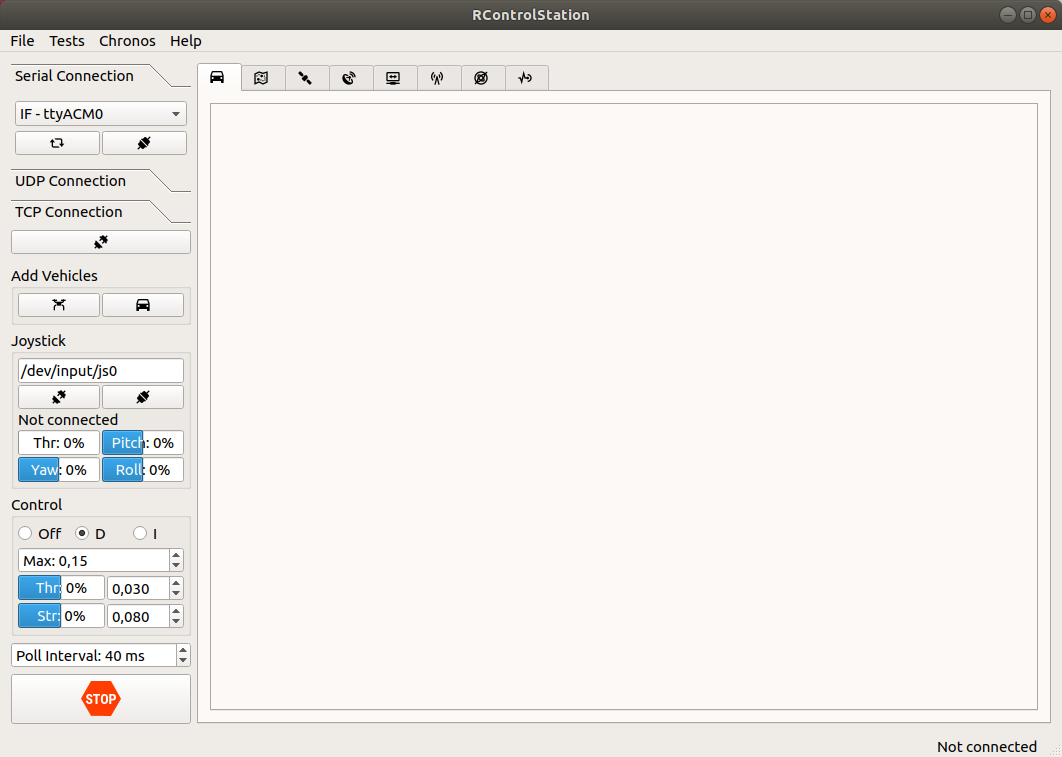
\includegraphics[width=0.7\textwidth]{./screens/RControlStation1.png}
    \end{center}
      
  \end{flushleft}\egroup
}
\makeatother


\newcommand{\GUIDEVERSION}[0]{$0.1$}
\newcommand{\GUIDETITLE}[0]{RISE Self Driving Vehicle Platform \newline \noindent
  Operator's Manual \newline \noindent Version: \GUIDEVERSION{}} 


\newenvironment{changeentry}[2]
               {
                 \noindent #1 : #2 \newline 
                 \vspace{2mm} \noindent
               }
               {
                 \vspace{2mm}
                 \hrule 
                 \vspace{2mm}
               }

\newcommand{\todo}[1]{{\color{red} \textbf{TODO:} #1}}
               


\begin{document}

\title{\GUIDETITLE}


\author{Benjamin Vedder\\ \texttt{benjamin.vedder@ri.se}\\ \vspace{5mm} Bo Joel Svensson\\ \texttt{joel.svensson@ri.se}} 

%  Use the @ symbol for simple inline code within prose:
\lstMakeShortInline[]@

\maketitle

%% \newpage

%% \section*{\small Disclaimer}

\newpage
\tableofcontents{}
\newpage


\section{Introduction}

This manual aims to outline and exemplify configuration and use of the
RISE Self Driving model Vehicle Platform (SDVP). It does not go in
depth in describing the hardware or software that run on the
microcontrollers in for example the RC car, but rather tries to give
just enough background for starting operate the system using the
RControlStation software which is a graphical user interface for
controlling and monitoring the SDVP.

RControlStation can, among much more, be used for the following:
\begin{itemize}
\item Track and trace movement of the SDVP overlaid on a map
  implemented based on OpenStreetMap.
\item Draw, load and save trajectories for the car to
  follow. Trajectories are visualised as line segments on the map.
\item Control the car directly via the keyboard.
\item Configure car dynamics.
\item Configure numerous parameters related to the positioning system.
\item monitor and log data obtained from the SDVP. 
\end{itemize} 


\todo{Write more here about what RControlStation is in an overview kind of way} 

\section{RISE SDVP Hardware Overview} 

The hardware found on the RC car consists of a motor controller (the
VESC), another controller board that call the RTK Controller and a
Raspberry Pi.  The Raspberry Pi is there to provide Wifi and/or 4G
cellular connectivity and enable for example remote debugging. The RTK
Controller implements the self driving aspects of the SDVP, includes
positioning capabilities using GPS and has two radios for
communication. The RTK Controller connects to the car steering servo,
providing its power and PWM signal for control. The RTK controller
connects to the VESC over CAN-bus. The Raspberry Pi is connected to
the RTK Controller over USB, it is possible to power the Pi through
this connection with a modification shown below.

\vspace{5mm}

\noindent \begin{minipage}{0.33\textwidth}
  \noindent 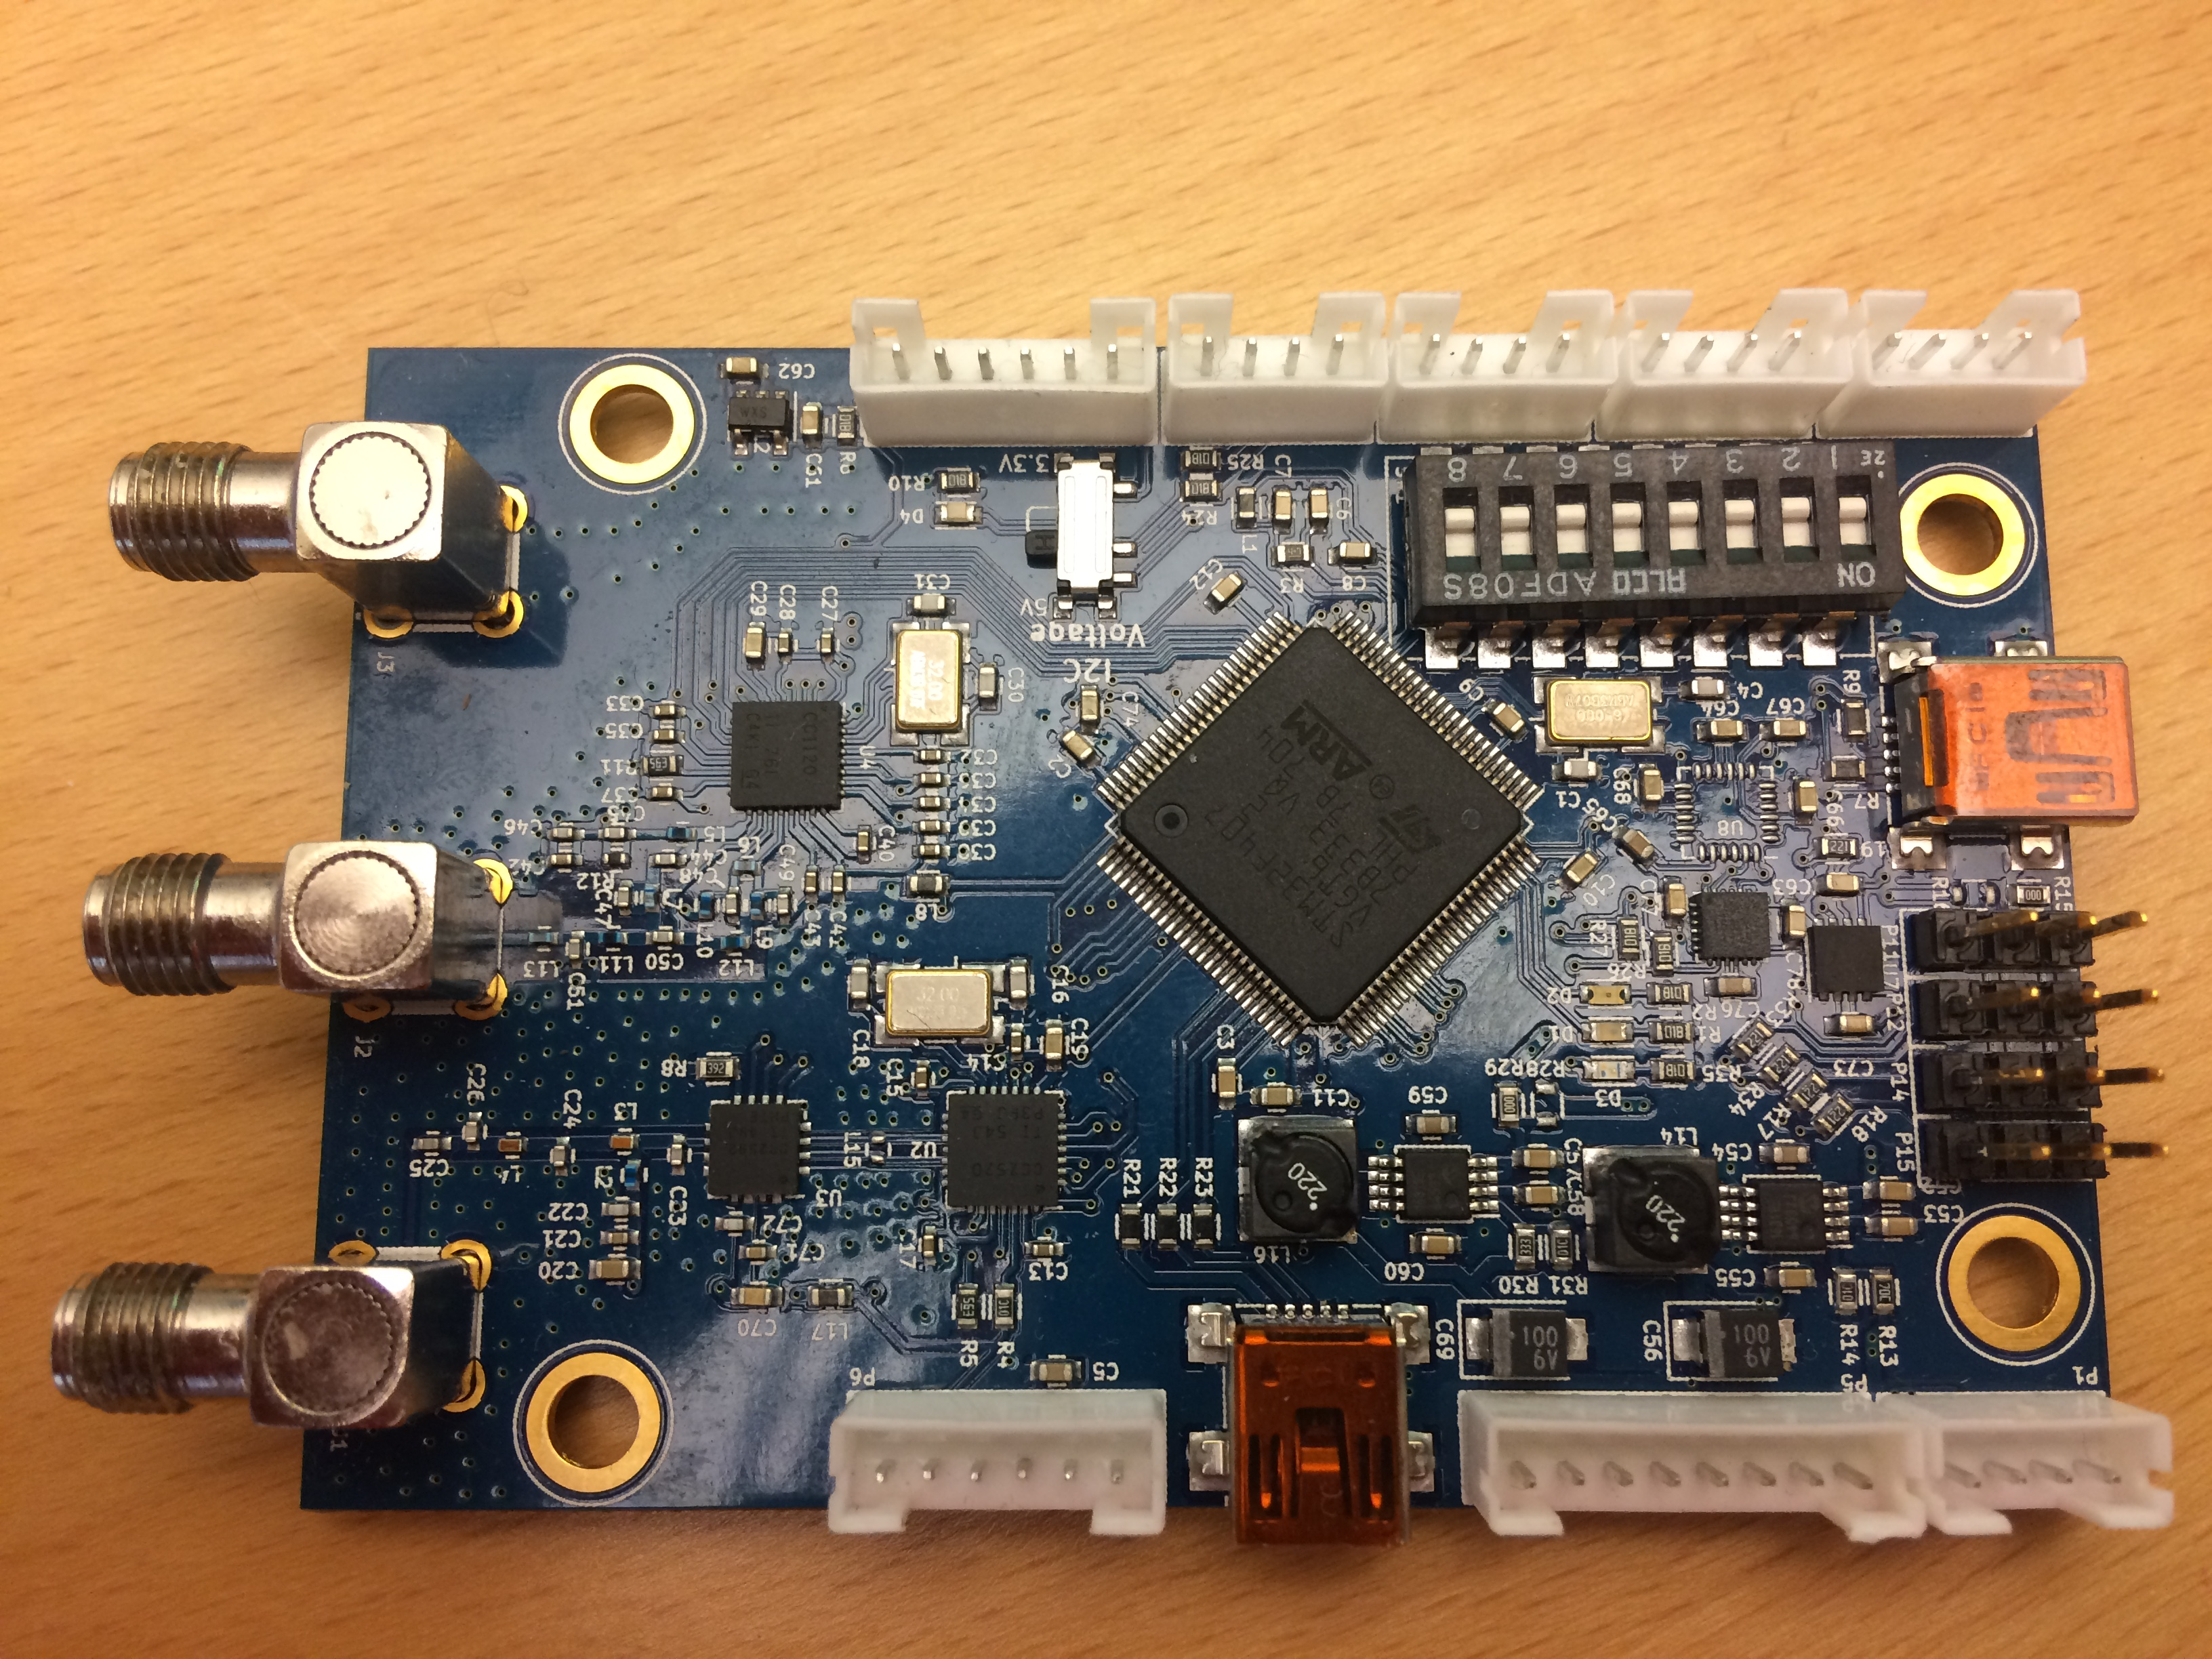
\includegraphics[width=\textwidth]{./photos/RTKControl2.JPG}
  \noindent 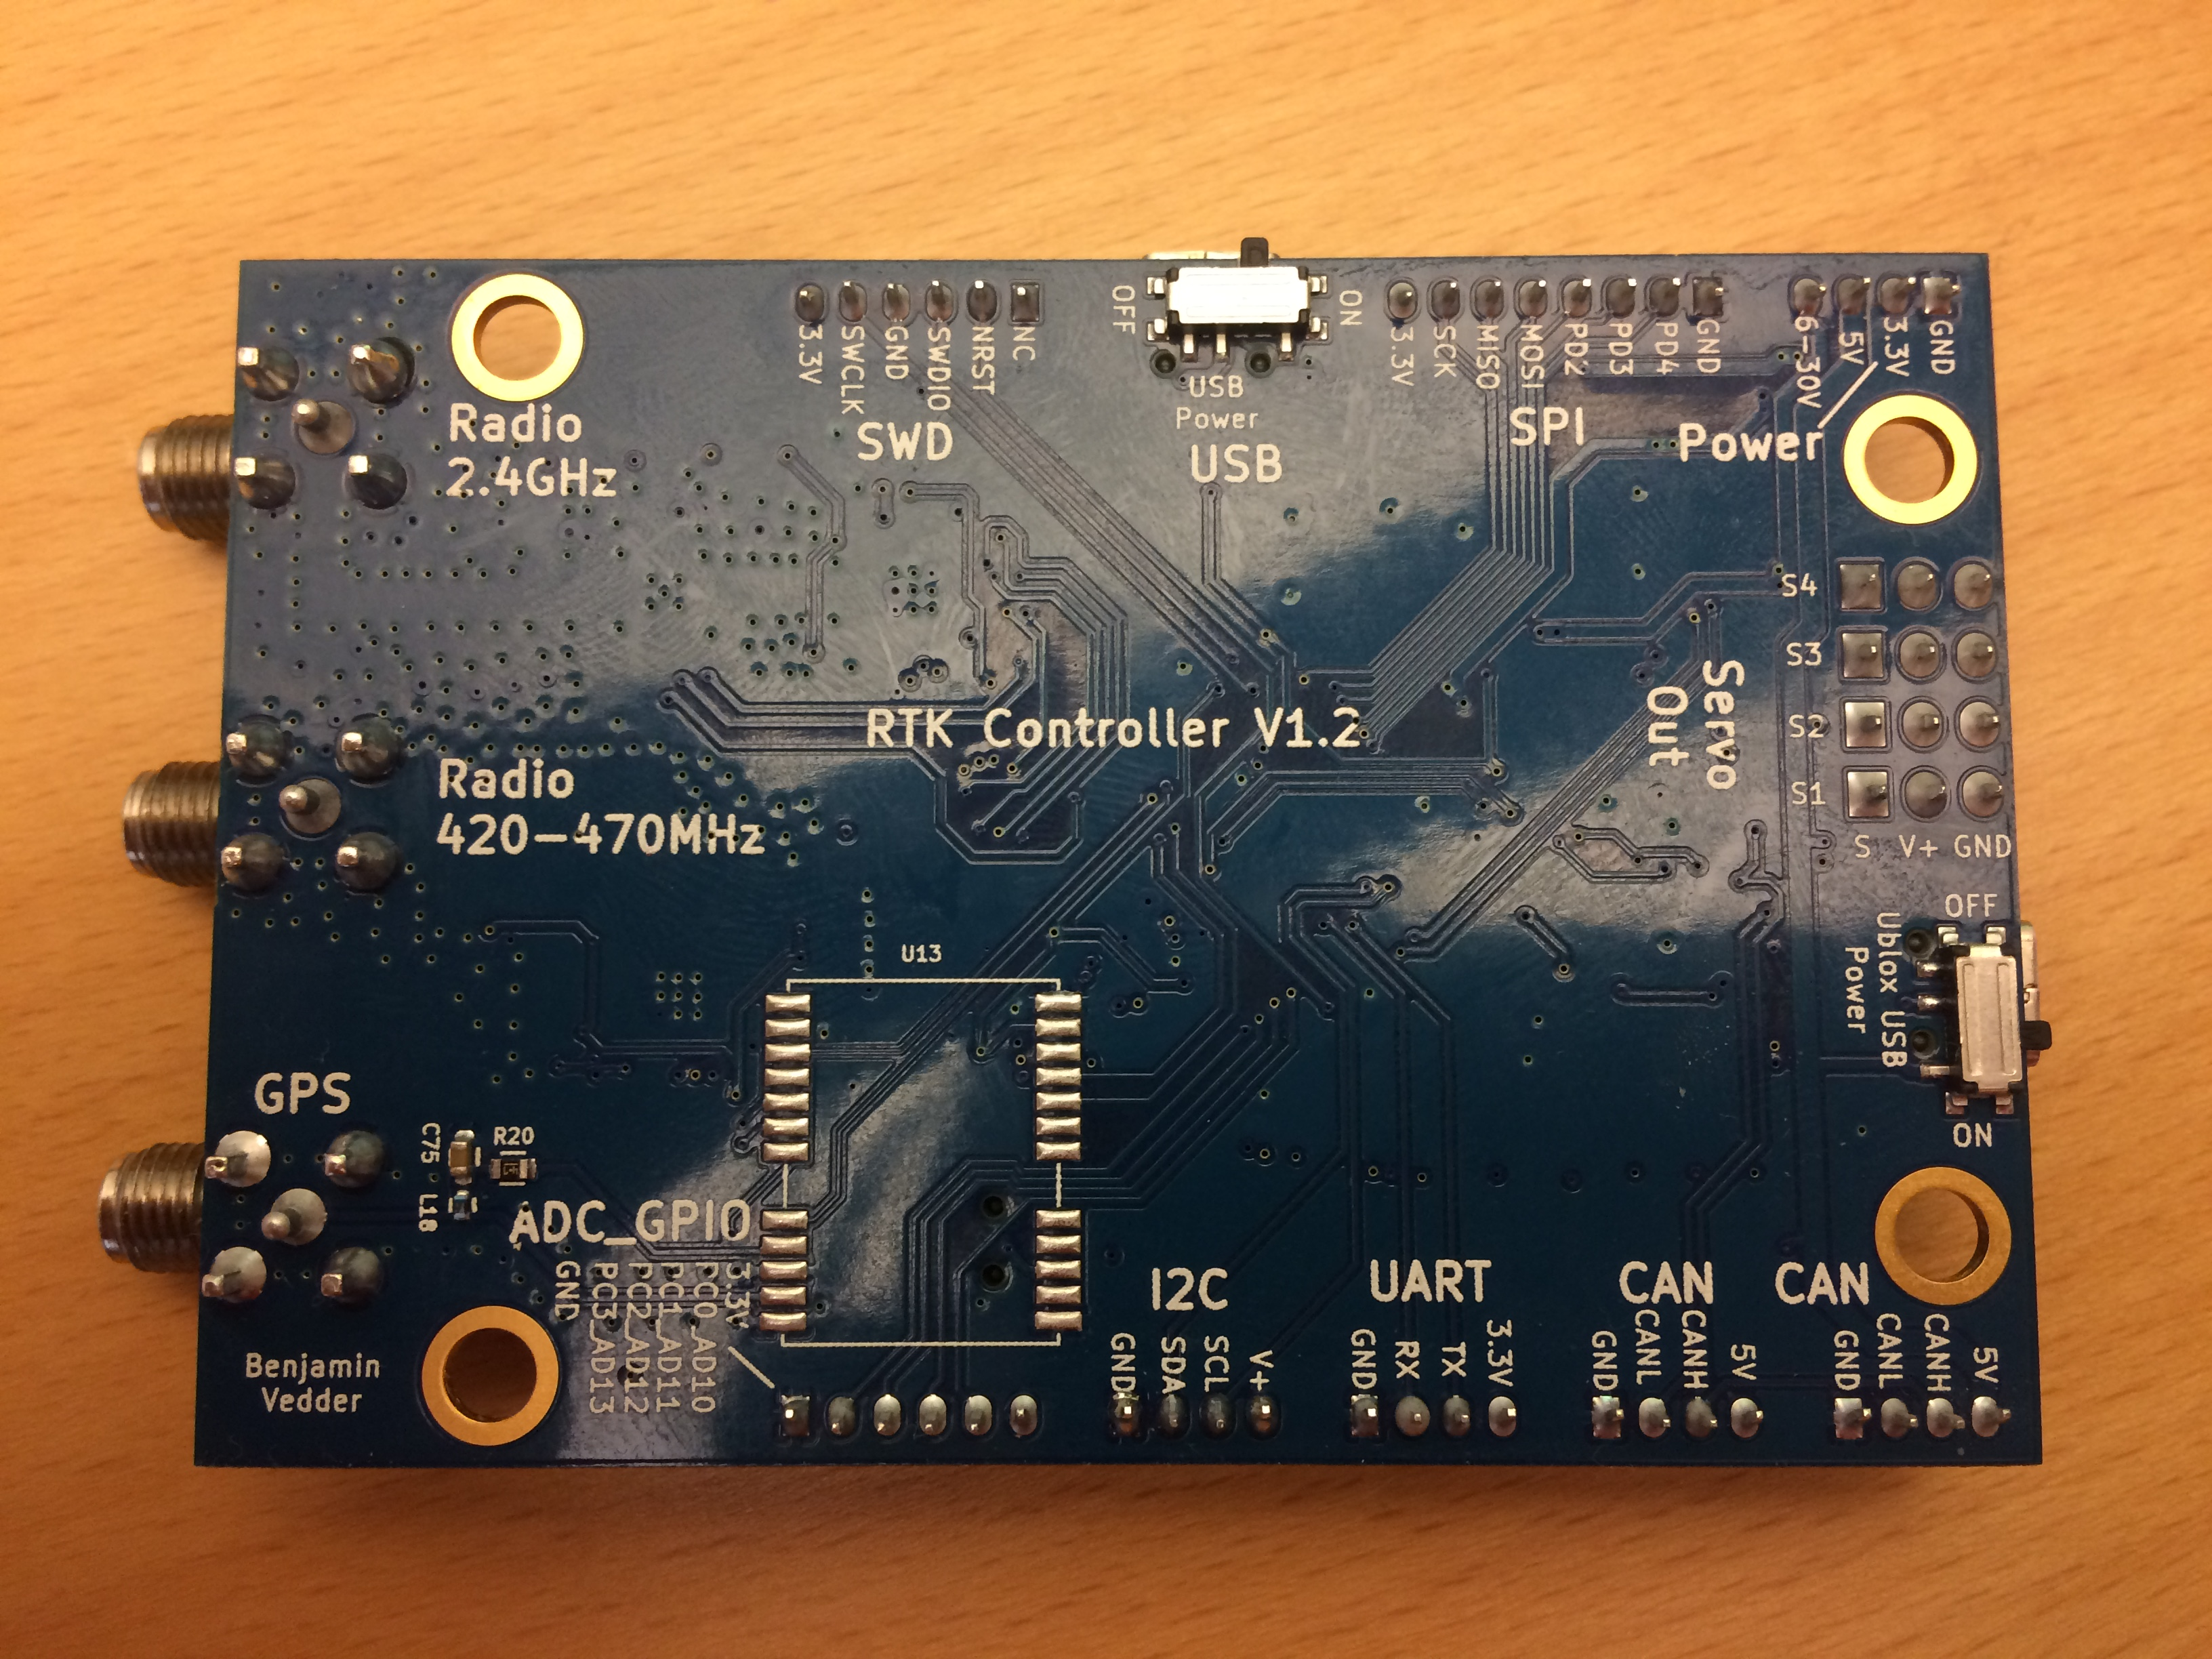
\includegraphics[width=\textwidth]{./photos/RTKControl1.JPG}
\end{minipage}
\begin{minipage}{0.66\textwidth} %% Text RTK
  The pictures show the top (top) and bottom (bottom) view of the RTK
  Controller. On the top view you can see three antenna connectors for
  GPS and radio.  There is a set of dip switches that configure the
  identity of the board. The set of connector pins along the right
  edge are for controlling servos and the write sockets are CAN, I2C,
  UART, SWD and SPI connectors.  On the bottom view you can see solder
  pads for a UBLOX chip (this card happens to not be equiped with one)
  and a small switch for toggling ``Power over USB'' to power a
  connected Raspberry Pi backwards through its USB port.  The RTK
  Controller connects to the computer running RControlStation either,
  over USB directly, over radio or over WIFI or 4G via the Raspberry
  Pi.
\end{minipage}

\vspace{5mm}

\noindent \begin{minipage}{0.66\textwidth} These pictures show the VESC
  motor controller, alone (top) and together with an RTK Controller
  and a motor (bottom). On the left side of the VESC (block of
  aluminium) you can see a battery connector.  On the other side of
  the aluminium are three cables for connecting a brushless motor.  On
  the bottom of the VESC there is also a set of connectors for CAN,
  SWD and so on. On the bottom picture, the RTK Controller is
  connected to the VESC over CAN.
  \todo{Insert information about max/min voltage} 
\end{minipage}
\begin{minipage}{0.33\textwidth} %% Text VESC
  \noindent 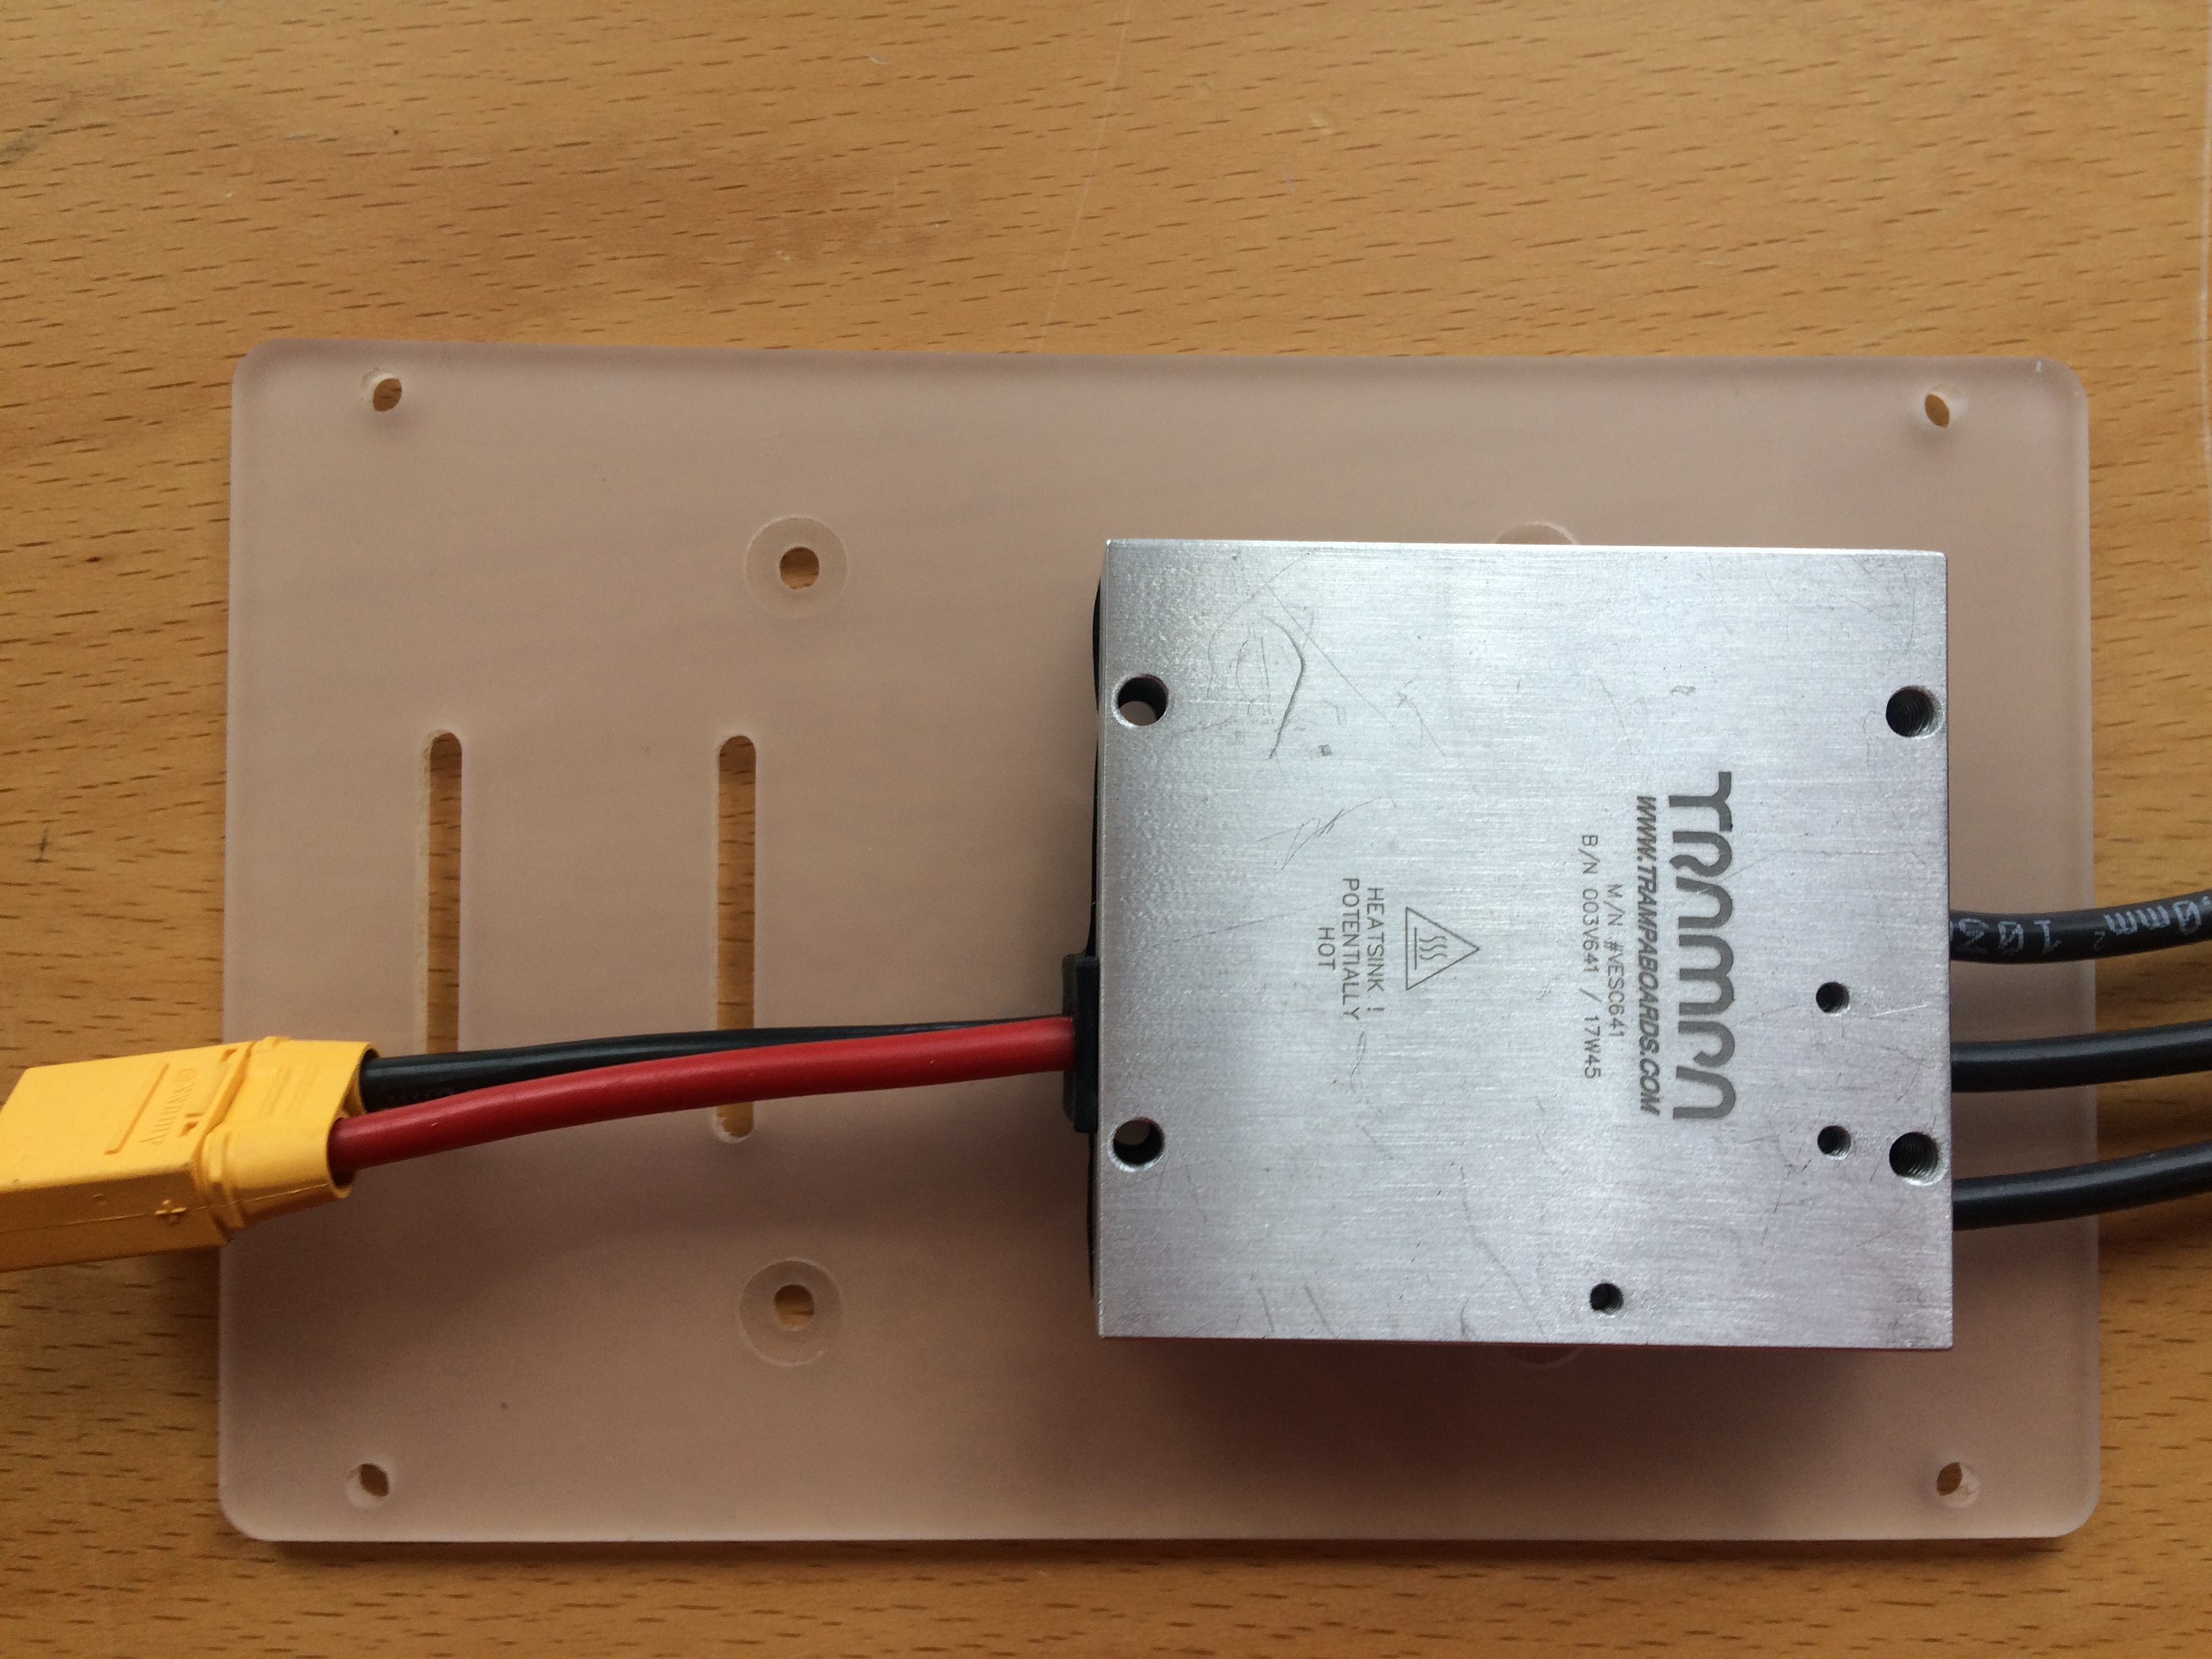
\includegraphics[width=\textwidth]{./photos/VESC.JPG}
  \noindent 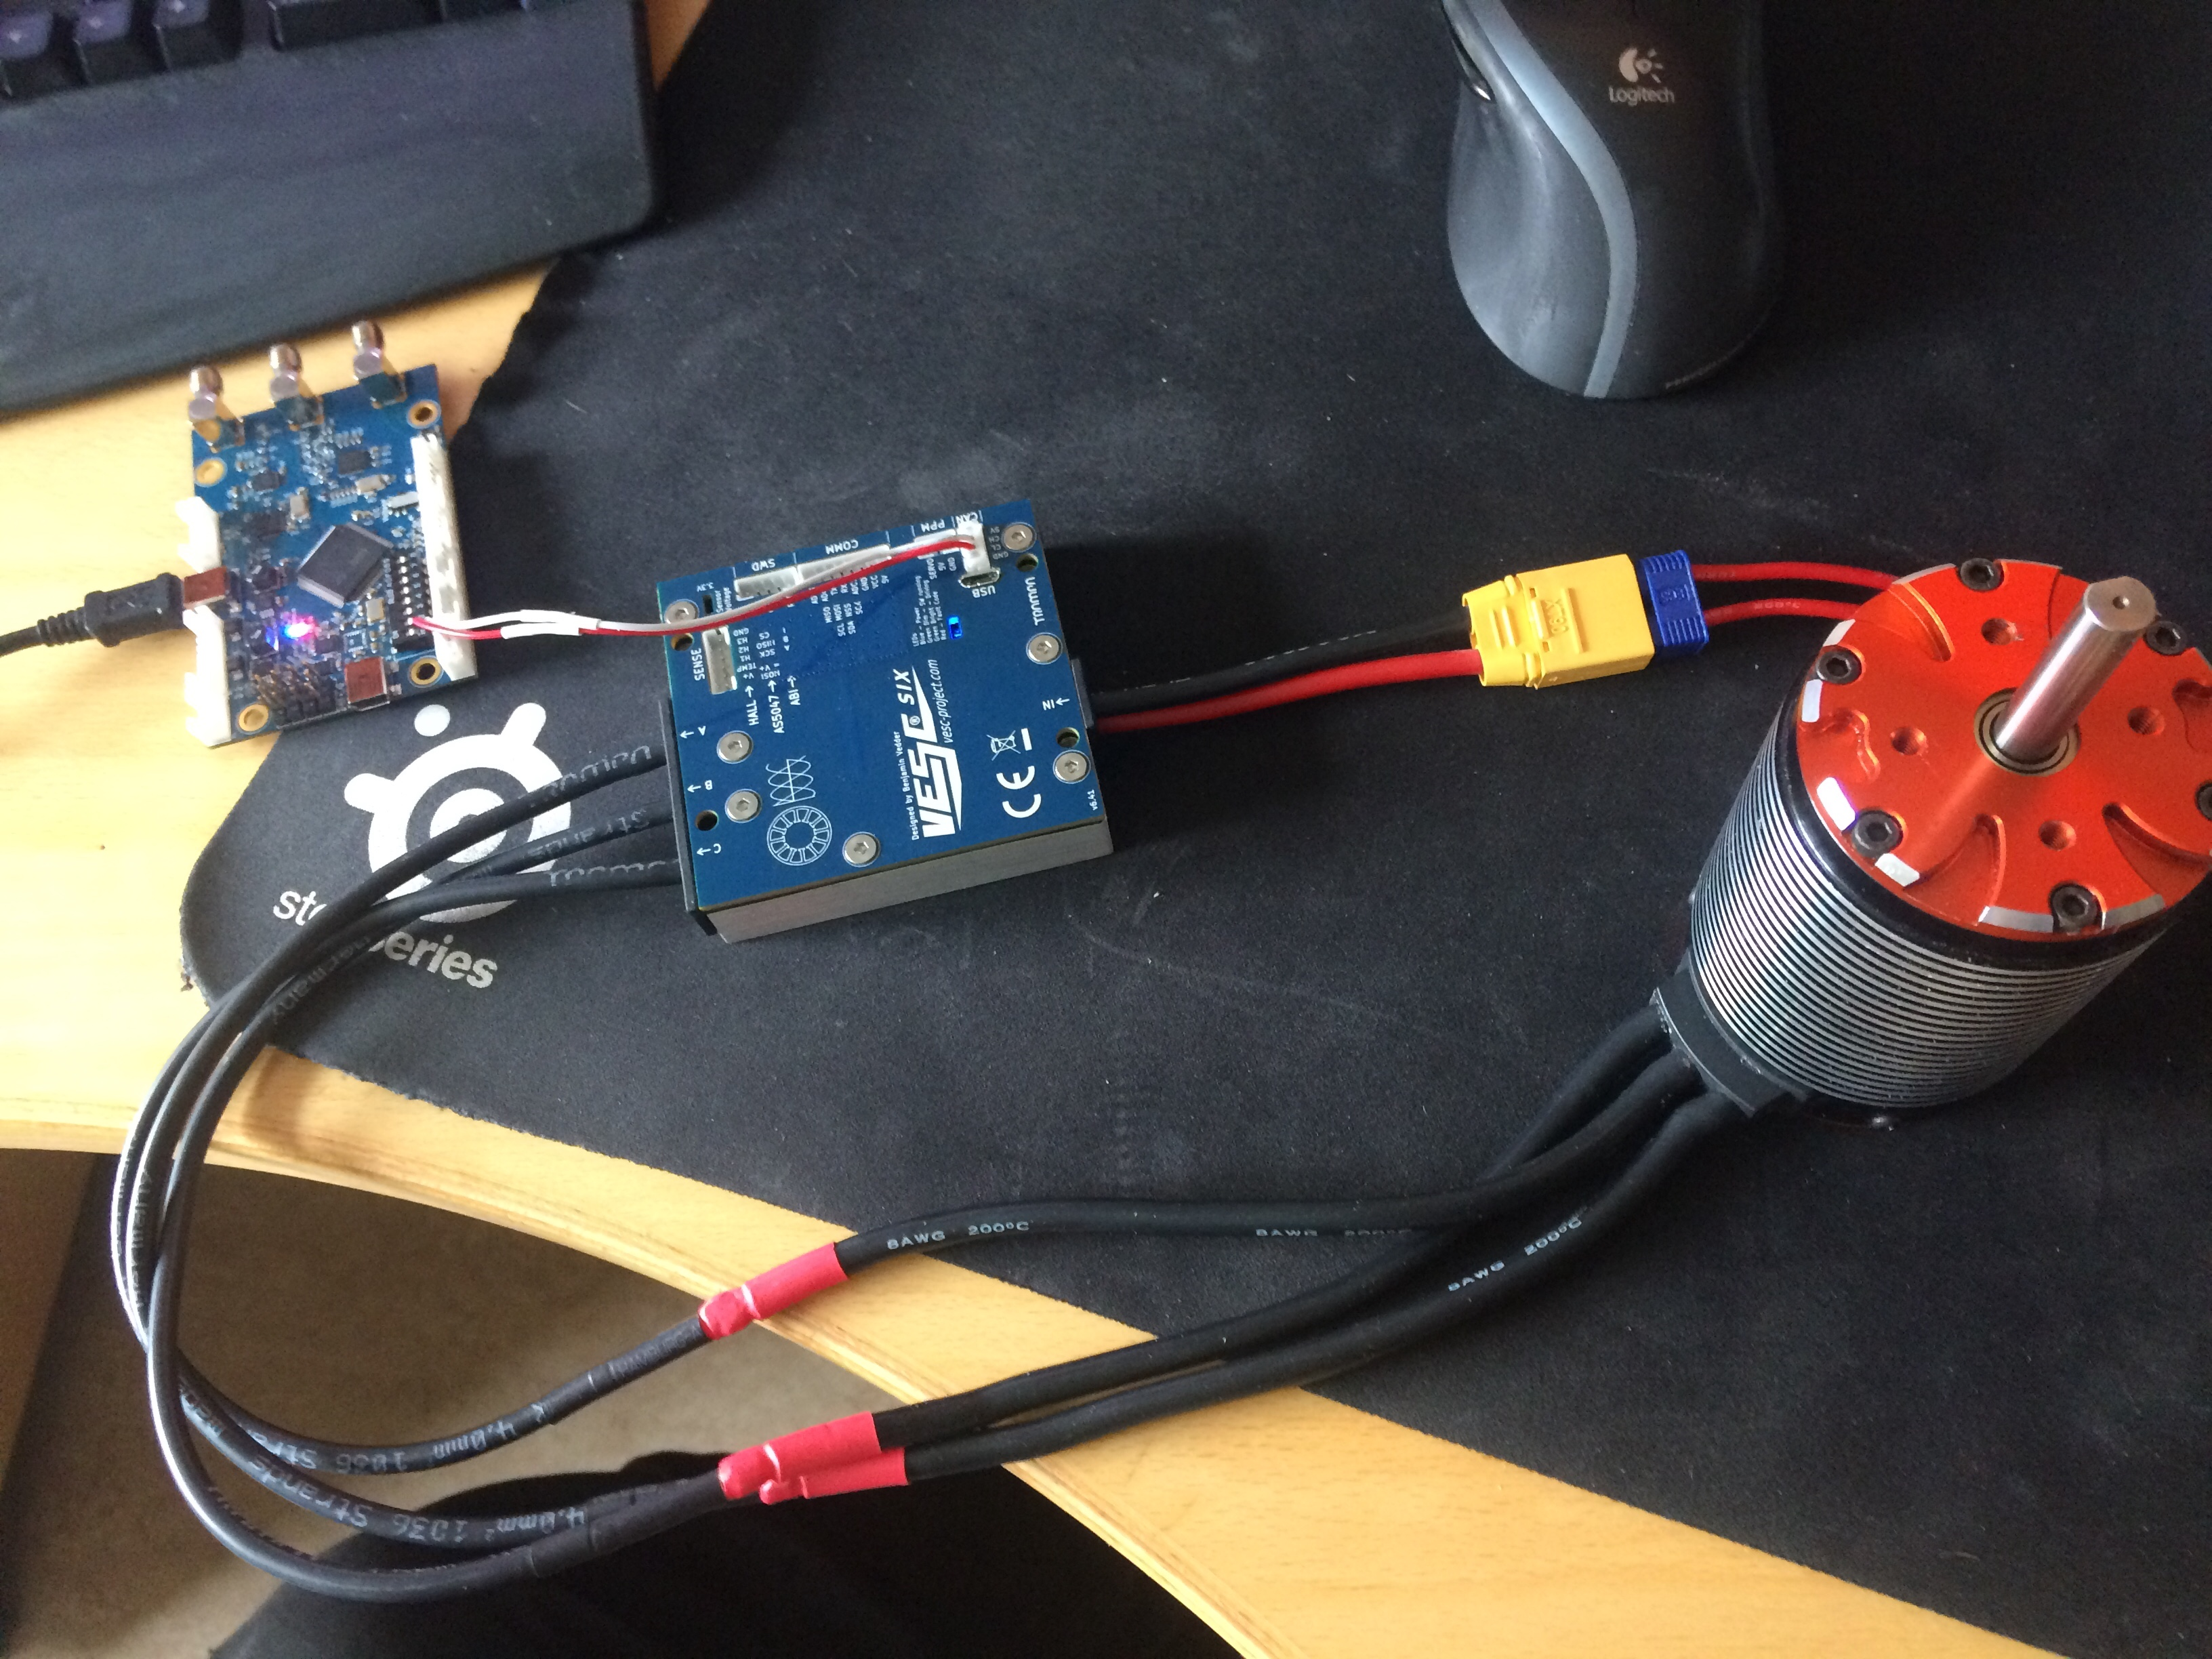
\includegraphics[width=\textwidth]{./photos/VESC_RTK.JPG}
\end{minipage}


\vspace{5mm}

\noindent \begin{minipage}{0.33\textwidth}
  \noindent 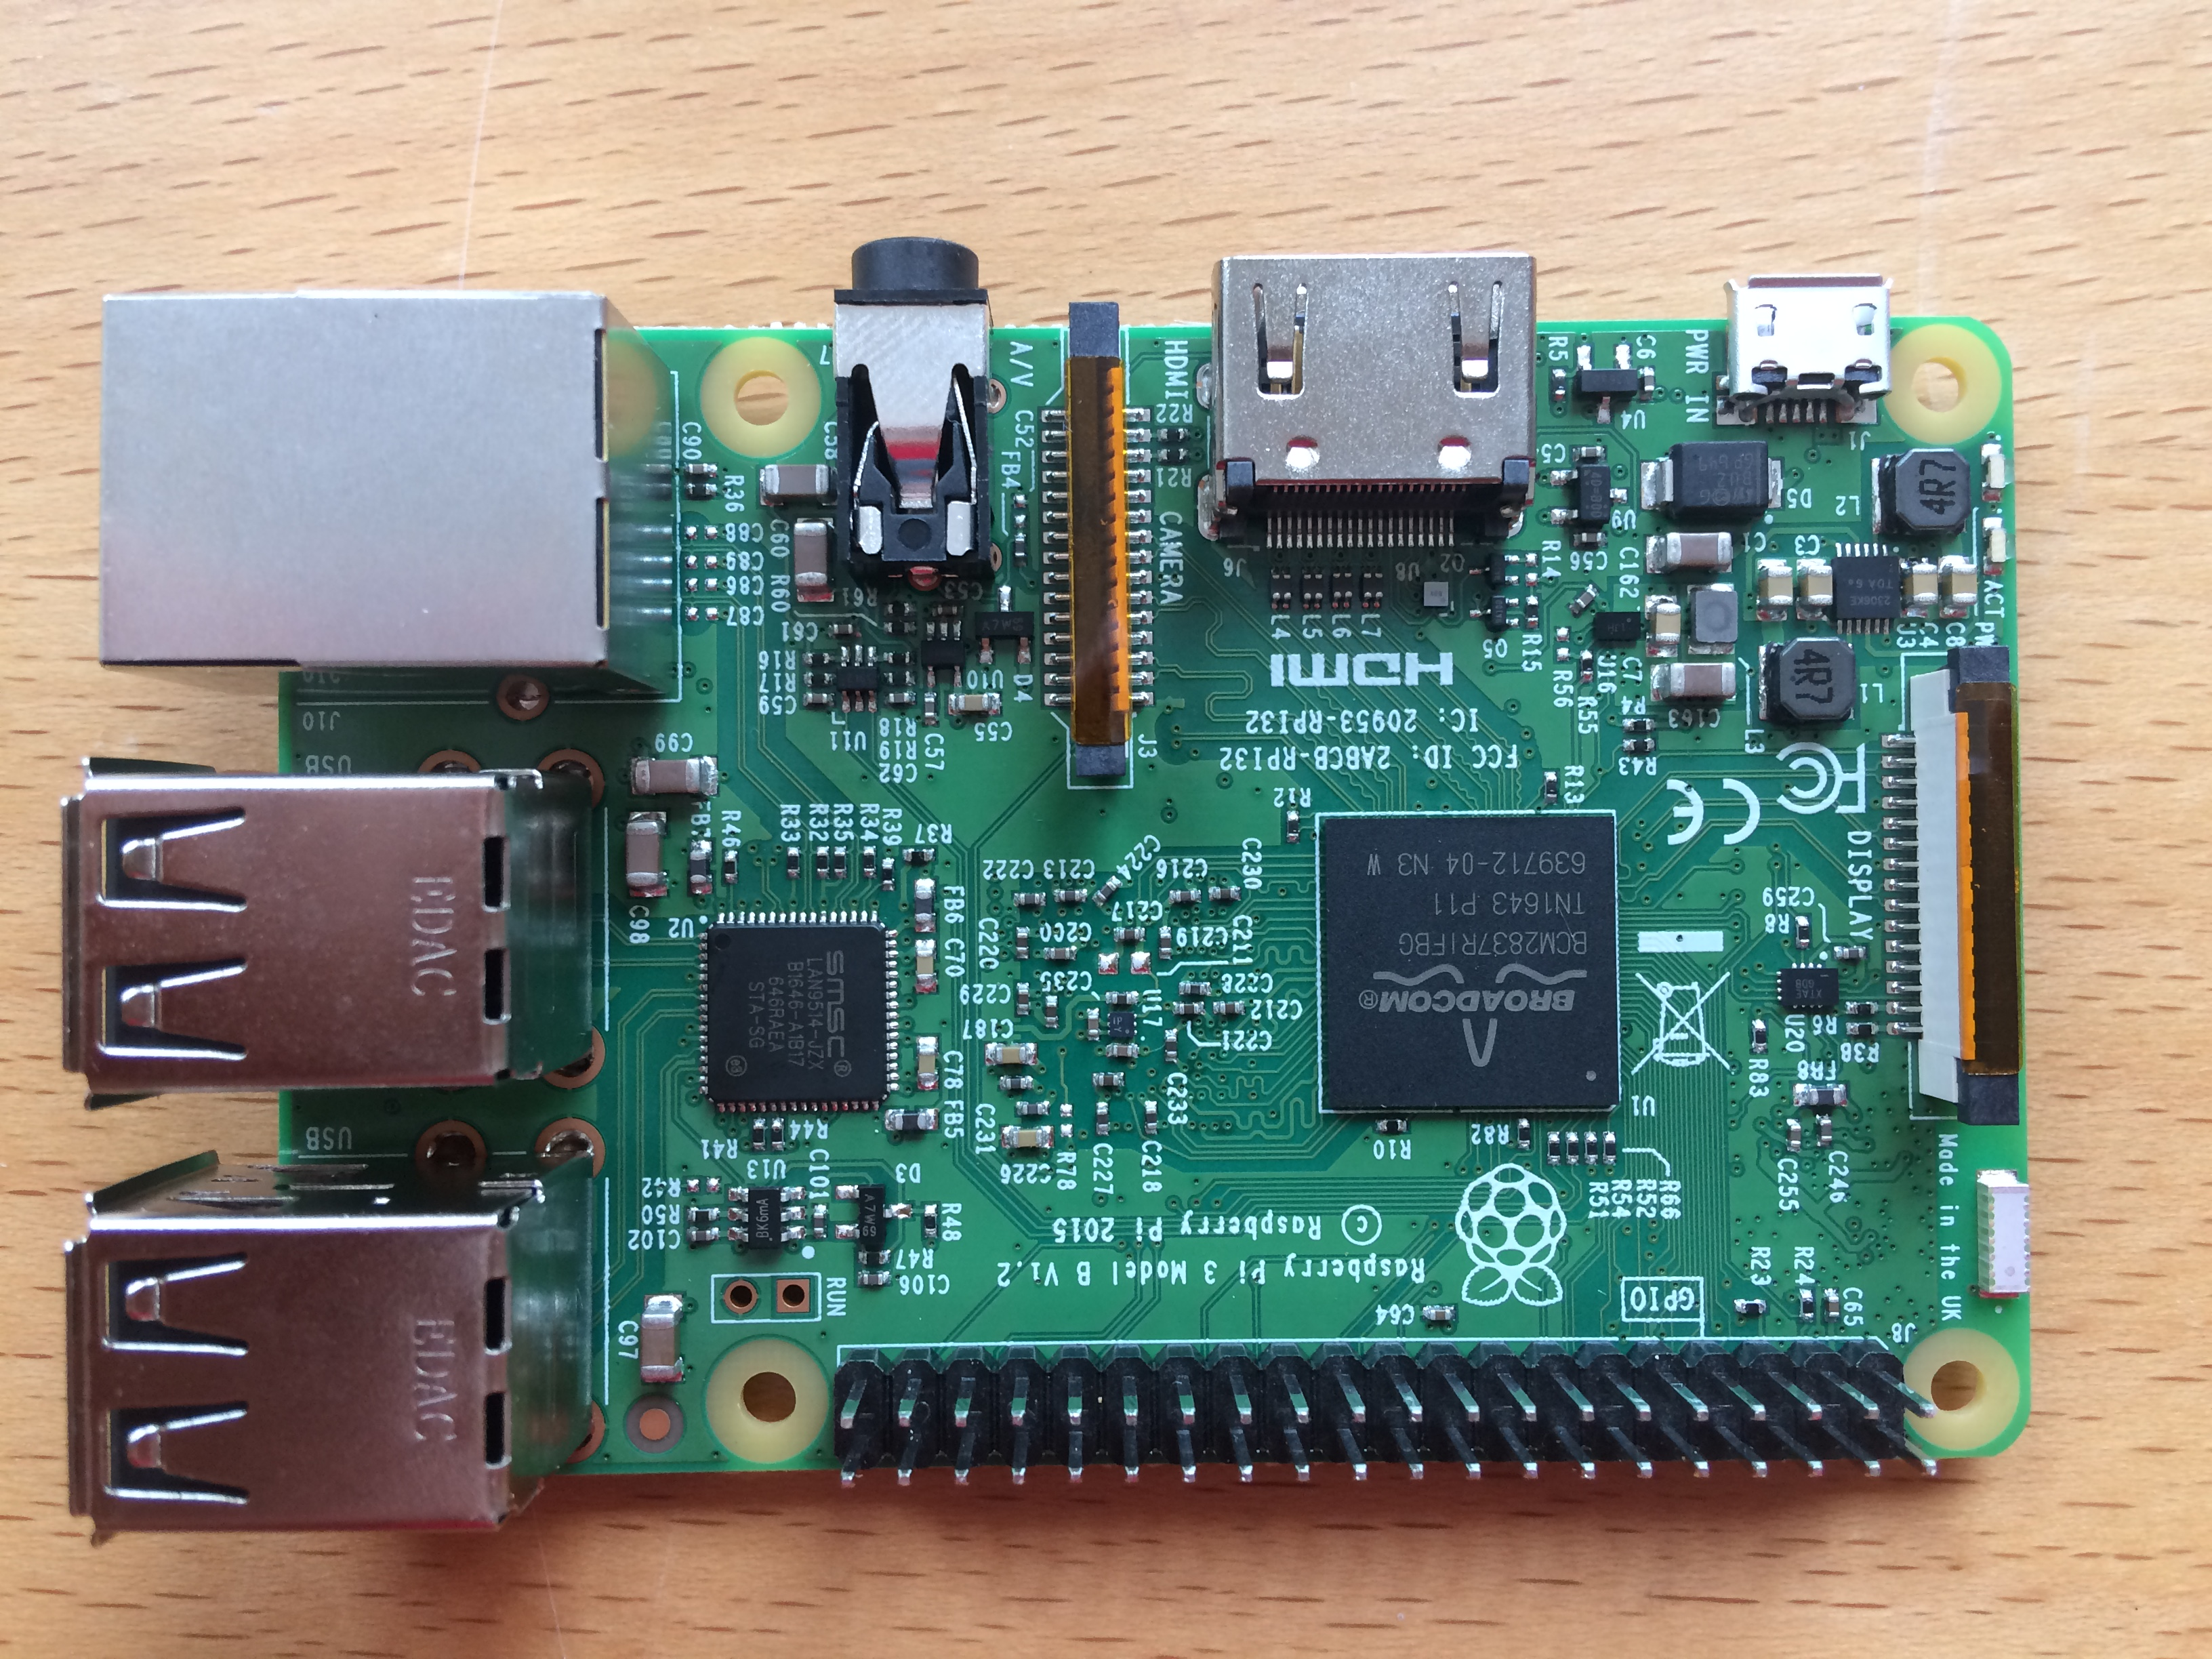
\includegraphics[width=\textwidth]{./photos/Pi1.JPG}
  \noindent 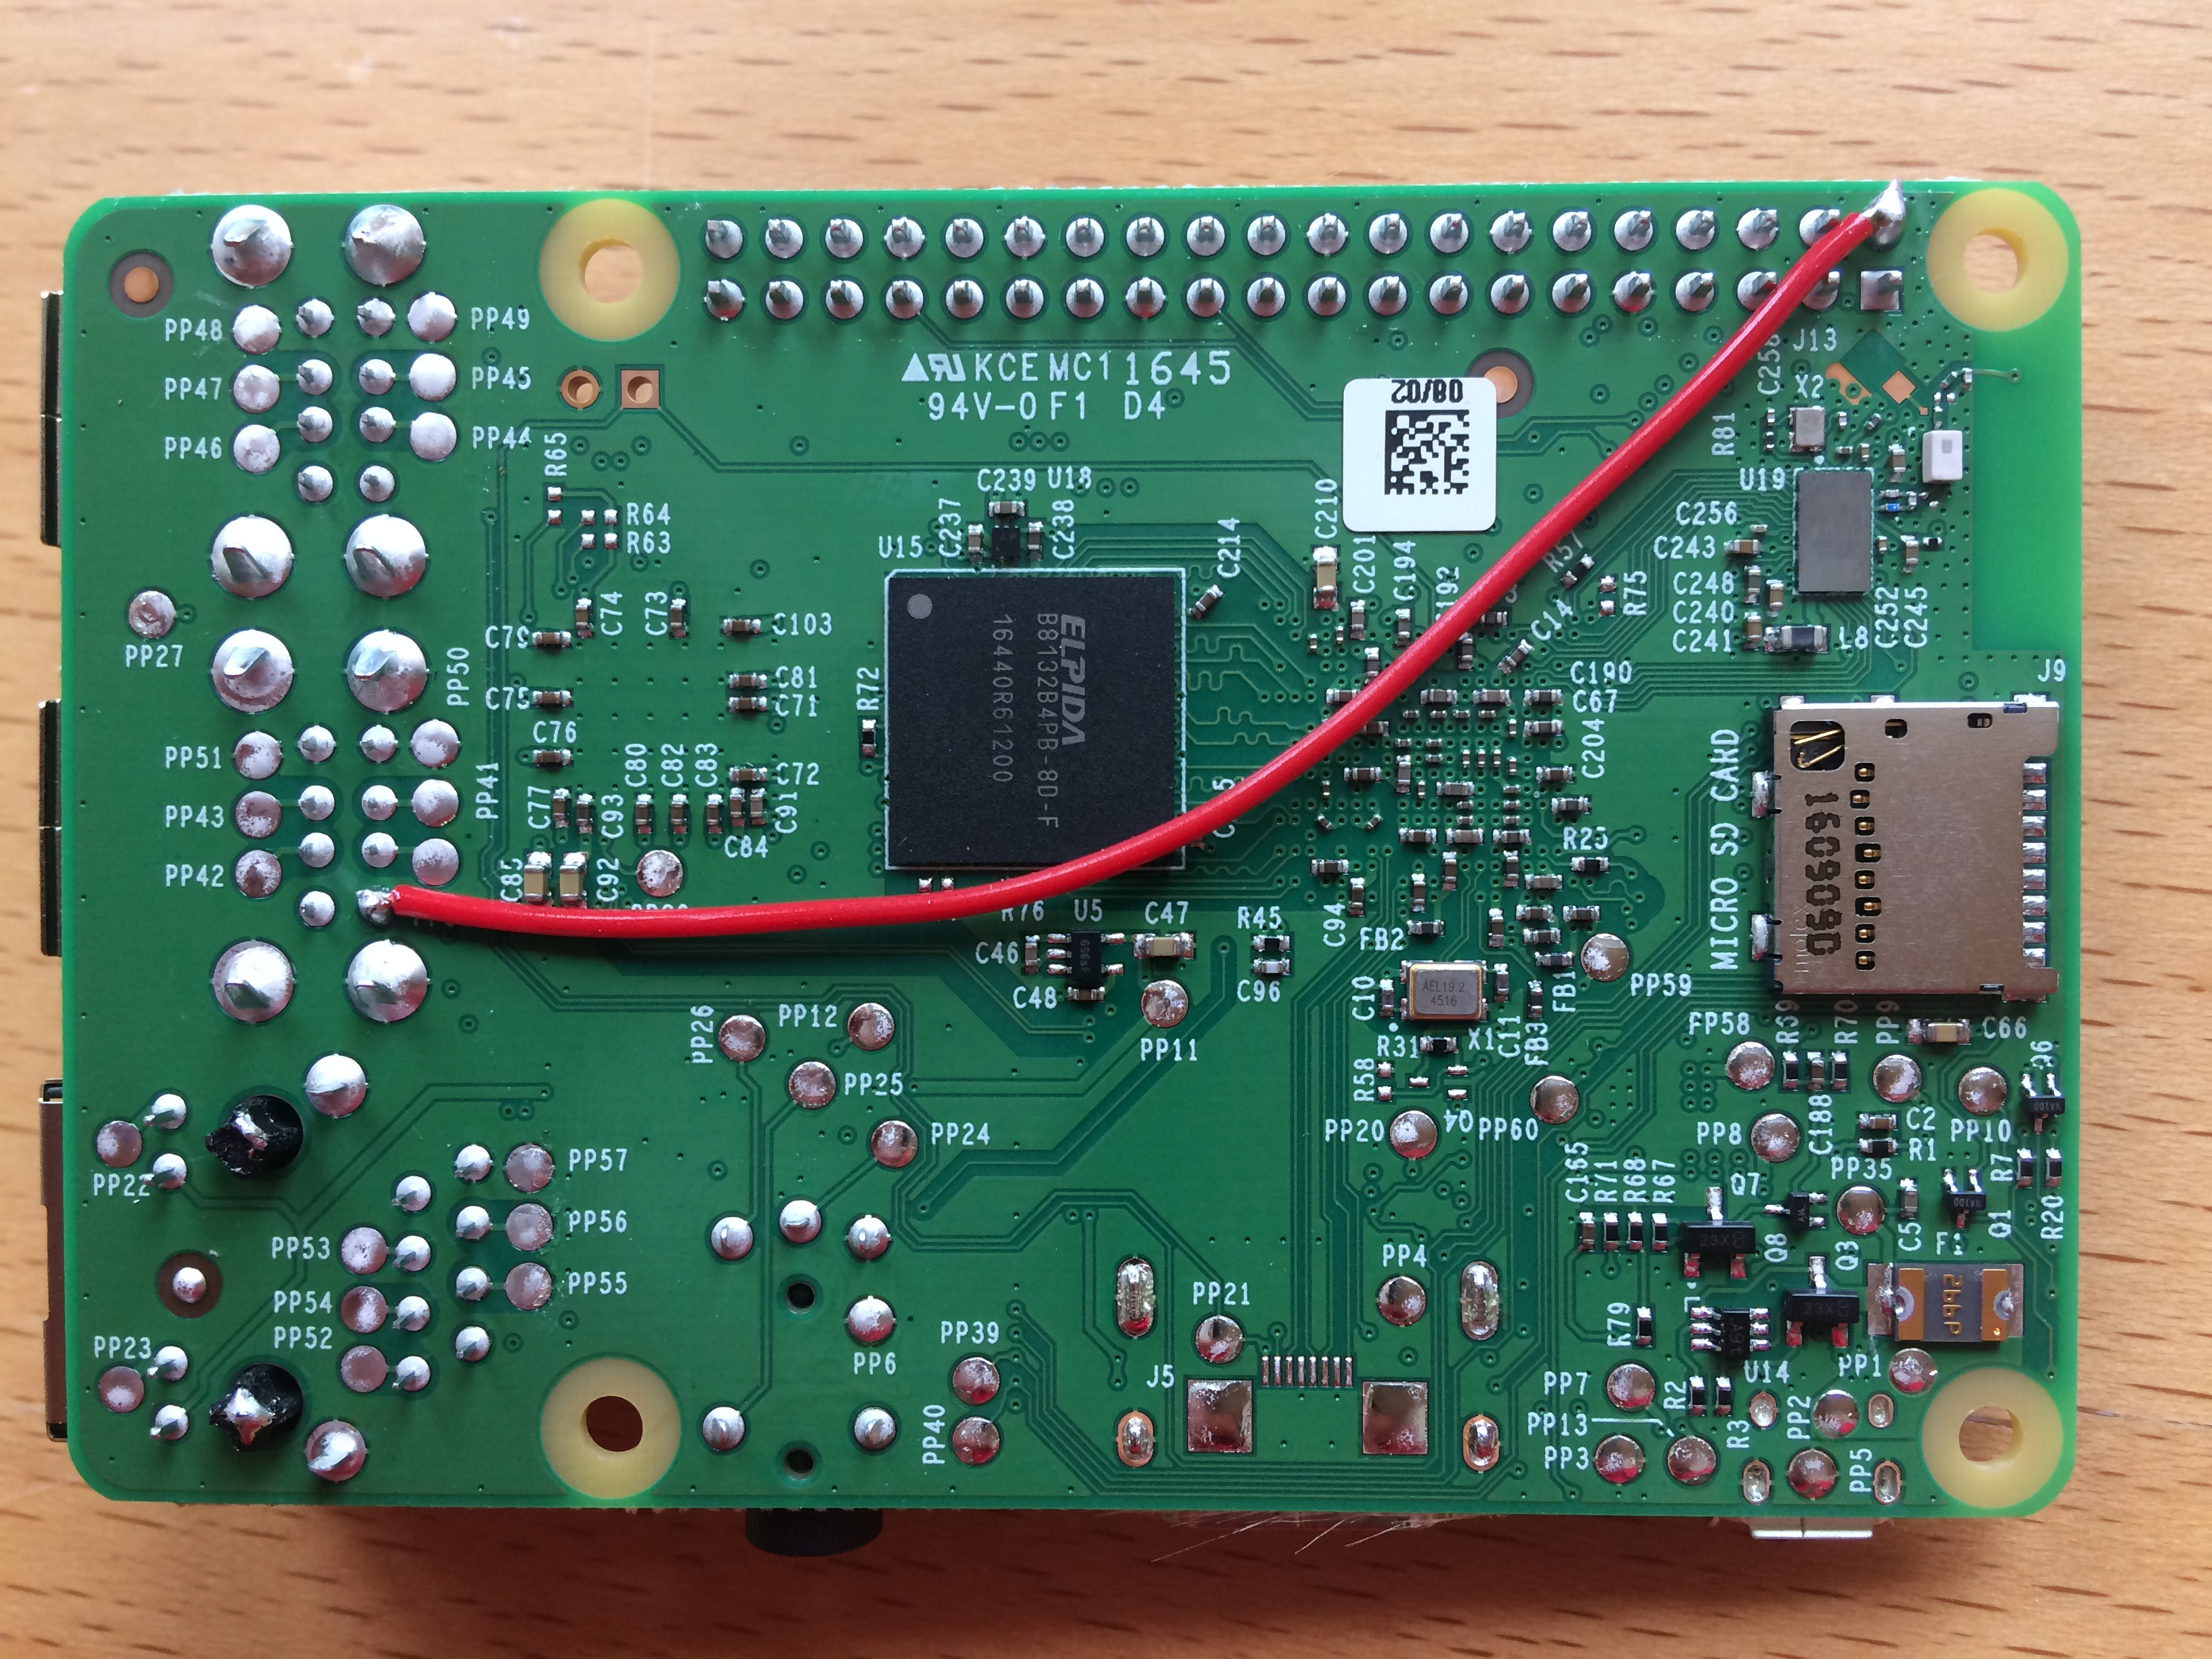
\includegraphics[width=\textwidth]{./photos/Pi2.JPG}
\end{minipage}
\begin{minipage}{0.66\textwidth} %% Text Modified raspberry pi
  These picture show a top and bottom view of a modified Raspberry
  Pi. The modification is a wire soldered from the 5V pin on the USB
  port to the Pi 5V net. The Pi's own voltage regulator transforms
  this to the 3.3V needed.
\end{minipage}

\todo{Maybe a picture of the little radio tranceiver (The mote?) ?}

\todo{A picture showing what features these provides and how they connect (something like in the paper)}


\section{Configuring a Linux Machine}

This section describes how to set up a linux system (an Ubuntu system
is assumed) with the tools needed to run RControlStation and to
develop towards the RISE SDVP. Start out by installing some basic
dependencies:

\begin{Verbatim}
\sudo apt-get install git build-essential libudev-dev
\end{Verbatim}

The IDEs (development environments) preferred by some of the authors of
this documentation is Qt-Creator and Eclipse. To download Eclipse
click
\href{http://ftp-stud.fht-esslingen.de/pub/Mirrors/eclipse/oomph/epp/photon/R/eclipse-inst-linux64.tar.gz}{here}
\footnote{\texttt{\tiny{wget
      http://ftp-stud.fht-esslingen.de/pub/Mirrors/eclipse/oomph/epp/photon/R/eclipse-inst-linux64.tar.gz}}}.
Qt can be downloaded from \url{https://www.qt.io/download} or click
\href{http://download.qt.io/official_releases/online_installers/qt-unified-linux-x64-online.run}{here}
to directly download the open source version. Now, install Qt and
Eclipse, both have install wizards to help with this procedure. 

Arm development tools are needed if you want to compile new versions
of the various firmwares for the microcontrollers on the
SDVP. Download arm development tools from \url{developer.arm.com} or
click this
\href{https://developer.arm.com/-/media/Files/downloads/gnu-rm/7-2018q2/gcc-arm-none-eabi-7-2018-q2-update-linux.tar.bz2?revision=bc2c96c0-14b5-4bb4-9f18-bceb4050fee7?product=GNU%20Arm%20Embedded%20Toolchain,64-bit,,Linux,7-2018-q2-update}{link}. 
  To install the ARM tools simply extract the files from the archive
  and place them in a suitable location, for example \texttt{\$HOME/opt/gcc-arm-none-eabi/}.
\begin{Verbatim}
  tar xvf gcc-arm-none-eabi-7-2018-q2-update-linux.tar.bz2
  mv gcc-arm-none-eabi-7-2018-q2-update-linux $HOME/opt/gcc-arm-none-eabi
\end{Verbatim} 
Then configure your \texttt{\$PATH} path variable to include \texttt{\$HOME/opt/gcc-arm-none-eabi/bin}

OpenOCD is used To flash the ARM Cortex M4 microcontrollers used throughout the SDVP.
To install OpenOCD execute the following command: 
\begin{Verbatim}
sudo apt-get install openocd
\end{Verbatim} 

Add yourself to the {\em dialout} group to be able to use, for example
{\texttt ttyACM0} without having to be root user (sudo). This is useful when connecting to
the various sdvp boards over a serial link (USB). 
\begin{Verbatim}
sudo usermod -a -G dialout <USER_NAME> 
\end{Verbatim}
After adding yourself to the dialout group, you need to log out and in again
for the change to take effect. 

It can also be good to uninstall modemmanager, if installed, as it sometimes leads to confusing the
system for a while when connecting over serial port.
\begin{Verbatim}
sudo apt-get remove modemmanager
\end{Verbatim}

Your Linux system is now set up for SDVP development (and use). The
next step is to clone the rise\_sdvp repository from github. Executing the
following command will create a new directory called rise\_sdvp, so make sure
are already in a suitable directory:
\begin{Verbatim}
cd <SUITABLE_DIR>   
git clone git@github.com:vedderb/rise_sdvp
\end{Verbatim}
The directory \texttt{<SUITABLE\_DIR>/rise\_sdvp} will in the rest of the document
be referred to as the \texttt{<SDVP\_DIR>}.


\section{Buidling RControlStation}

To build and run RControlStation, start Qt-Creator and on the welcome
screen click {\em Open Project}. Navigate in the directory hierarchy
to where you cloned the rise\_sdvp repository and go to
\texttt{<SDVP\_DIR>/Linux/RControlStation}. Select the file
\texttt{RControlStation.pro} and click open. Qt-Creator will now open
the project and switch to a new view that allows you to edit files.
On the left side of the window you can browse the RControlStation
project.  To build, locate the {\em Build} menu and select {\em Build
  Project ``RControlStation''}.  At the bottom of the Qt-Creator
window there is a collection of tabs, one of them reads {\em 4 Compile
  Output}. You can keep an eye on this tab for any error outputs
during compilation. 

When compilation concludes successfully, click the little green
``play'' button located along the left edge of Qt-Creator. This should
bring up RControlStation.

\section{RControlStation GUI}

When RControlStation starts up you should be presented with a view very similar to
this:
\noindent 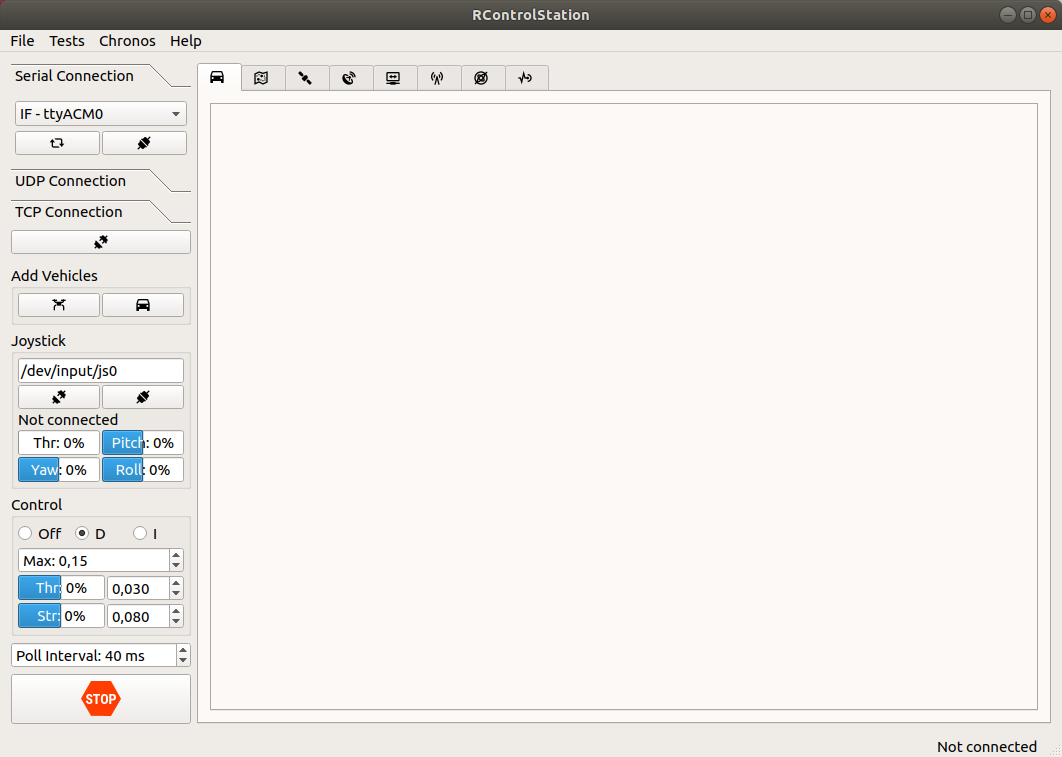
\includegraphics[width=\textwidth]{./screens/RControlStation1.png}
In this section we will go through and briefly explain the meaning and functionality
behind most of the elements of this GUI.

%\subsection{Menu Bar}

%\noindent 
\includegraphics[width=0.3\textwidth]{./screens/menubar1.png}
%It just feels silly to try and explain this. 


%% \noindent {\bf File:} 
%% \begin{itemize}
%% \item Save Routes
%% \item Save Routes with IDs
%% \item Load Routes
%% \item Exit
%% \end{itemize}

%% \noindent {\bf Tests:}
%% \begin{itemize}
%% \item Intersection
%% \item GPS Simulator
%% \end{itemize} 

%% \noindent {\bf Chronos:}
%% \begin{itemize}
%% \item Save selected route as drive file
%% \item Load drive file
%% \end{itemize}

%% \noindent {\bf Help:}
%% \begin{itemize}
%% \item About
%% \item About Libraries Used
%% \item About Qt
%% \end{itemize}



\subsection{Connectivity Controls}


\noindent \begin{minipage}{0.2\textwidth}
  \noindent 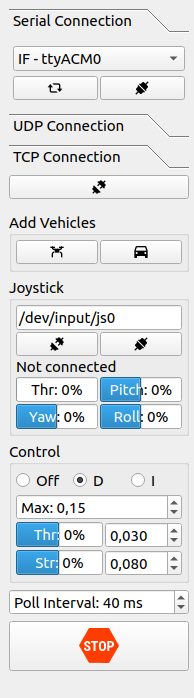
\includegraphics[width=\textwidth]{./screens/Left_controls1.png}
\end{minipage}
\begin{minipage}{0.7\textwidth}
  To the left side of RControlStation are fields for selection method of connecting to the
  SDVP, adding vehicles and control related configuration and indicators.  
  \begin{itemize}
  \item {\bf Connection:} Serial, UDP or TCP connection can be
    selected. Serial is used when connecting to the RTK controller
    using the radio mote or directly via USB cable. UDP and TCP
    connects to the SDVP via Raspberry Pi using either WIFI or 4G.
    Below the connection tabs is a button for disconnecting whatever
    connection has been set up. 
  \item {\bf Add Vehicles:} Add a car or quadcopter. Adding for
    example a car, changes the view on the right side to display a car
    and its set of car specific controls. The car specific controls are
    shown in Section~\ref{sec:cars} and quadcopter controls in Section\ref{sec:quads}.
  \item {\bf Joystick:} 
  \item {\bf Control:} Is related to the keyboard control
    functionality. It can be turned off, put in ``D'' mode or ``I''
    mode. ``D'' refers to duty mode and ``I'' representing current
    mode.  A ``gain'' value can be set for thrust and steering that
    influences how strongly these respond to keyboard interaction.
  \item {\bf Poll Interval:}
  \item {\bf Stop:} Stops a moving car. \todo{improve} 
  \end{itemize} 
\end{minipage}


\subsection{Cars}
\label{sec:cars}

%% ------------------------------------------------------------
\begin{minipage}{0.5\textwidth}
    \noindent 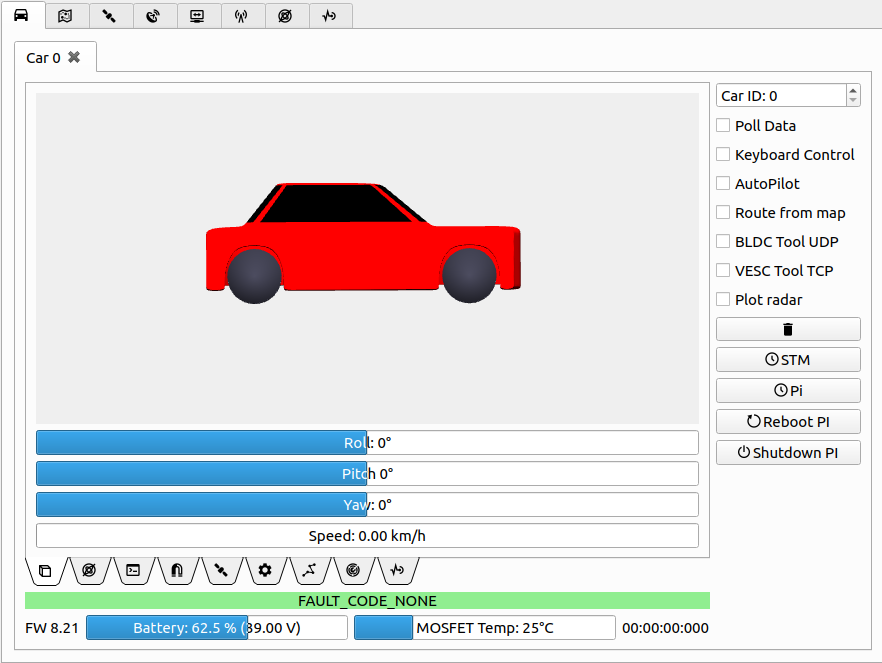
\includegraphics[width=\textwidth]{./screens/Car_orientation.png}
\end{minipage}
\begin{minipage}{0.5\textwidth} %% Text Car orientatio
  After adding a car, ``Car 0'' will appear in the Cars tab with a set
  controls similar to this image.  The ``Car ID'' field should be set
  so that it corresponds to the setting of the dip switches on the RTK
  controller. A way to test if the connection to the car is working,
  is to check the {\bf Poll data} box and checking if the picture of
  the car seems to respond to moving of the actual car.

  {\bf Keyboard Control}

  {\bf AutoPilot}

  {\bf Route from map}

  {\bf BLDC Tool UDP}

  {\bf VESC Tool TCP}

  {\bf Plot radar}
  
\end{minipage}
%% ------------------------------------------------------------


%% ------------------------------------------------------------
\begin{minipage}{0.5\textwidth} %% Text Car IMU
  \todo{text imu}      
\end{minipage}
\begin{minipage}{0.5\textwidth}
      \noindent 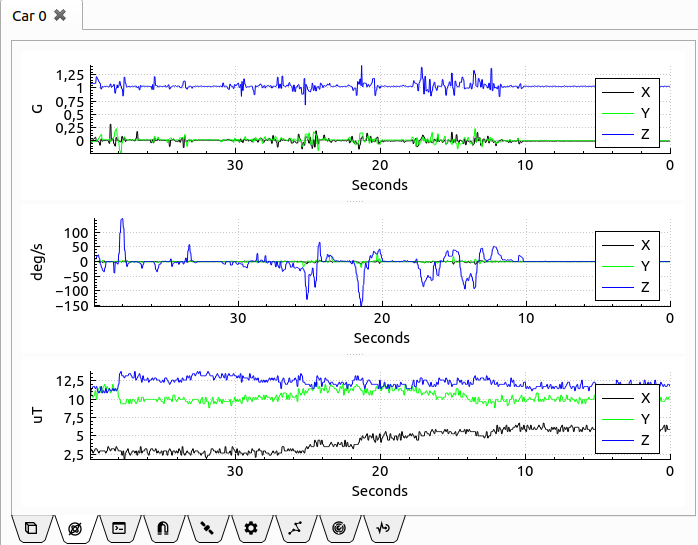
\includegraphics[width=\textwidth]{./screens/Car_IMU_realtime.png}
\end{minipage}
%% ------------------------------------------------------------


%% ------------------------------------------------------------
\begin{minipage}{0.5\textwidth}
  \noindent 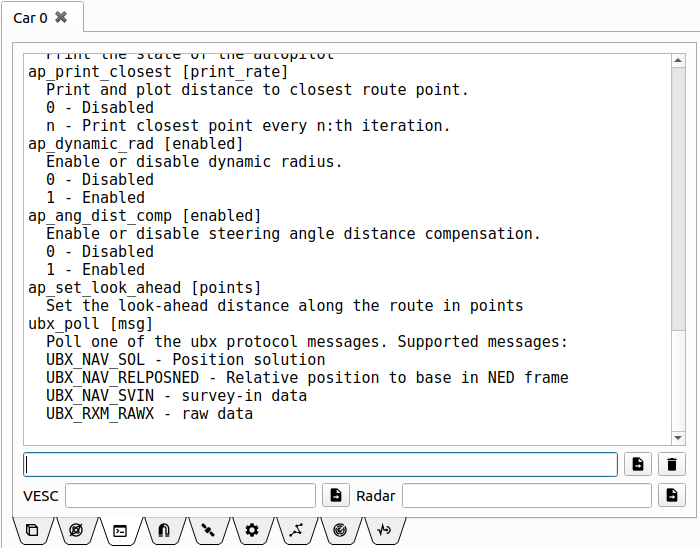
\includegraphics[width=\textwidth]{./screens/Car_terminal.png}
\end{minipage}
\begin{minipage}{0.5\textwidth} %% Text Car IMU
  \todo{text}
\end{minipage}

%% ------------------------------------------------------------


%% ------------------------------------------------------------
\begin{minipage}{0.5\textwidth} %% Text Car calibration
  \todo{text}
\end{minipage}
\begin{minipage}{0.5\textwidth}
  \noindent 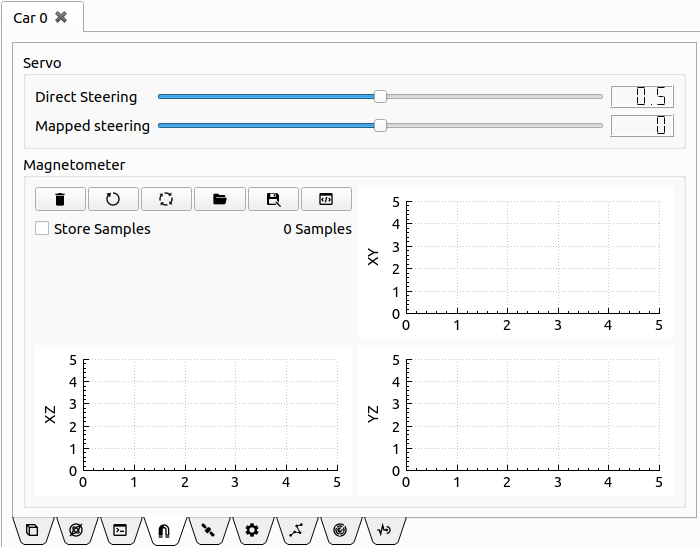
\includegraphics[width=\textwidth]{./screens/Car_calibration.png}
\end{minipage}
%% ------------------------------------------------------------

%% ------------------------------------------------------------
\begin{minipage}{0.5\textwidth}
  \noindent 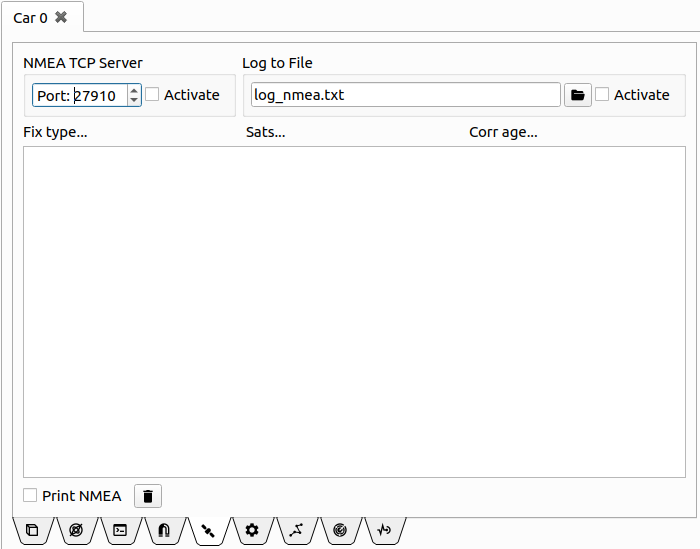
\includegraphics[width=\textwidth]{./screens/Car_GPS.png}
\end{minipage}
\begin{minipage}{0.5\textwidth} %% Text Car GPS
  \todo{text}
\end{minipage}
%% ------------------------------------------------------------

%% ------------------------------------------------------------
\begin{minipage}{0.5\textwidth} %% Text Car Configuration
  \todo{text}
\end{minipage}
\begin{minipage}{0.5\textwidth}
  \noindent 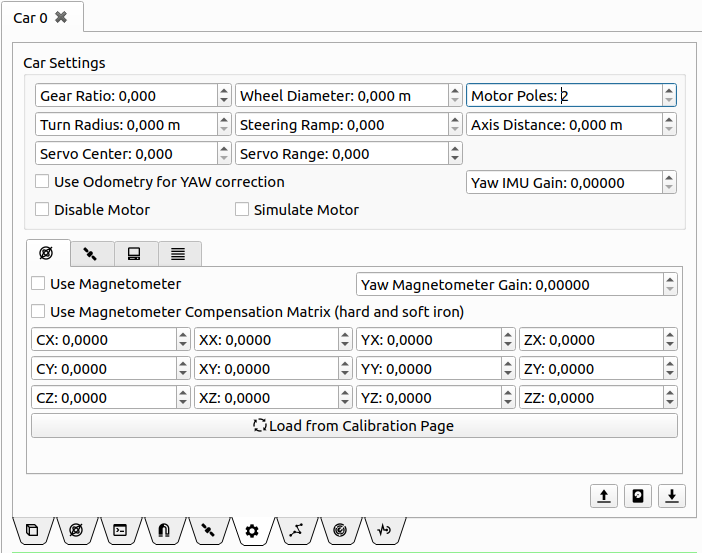
\includegraphics[width=\textwidth]{./screens/Car_configuration.png}
\end{minipage}
%% ------------------------------------------------------------


%% ------------------------------------------------------------
\begin{minipage}{0.5\textwidth}
  \noindent 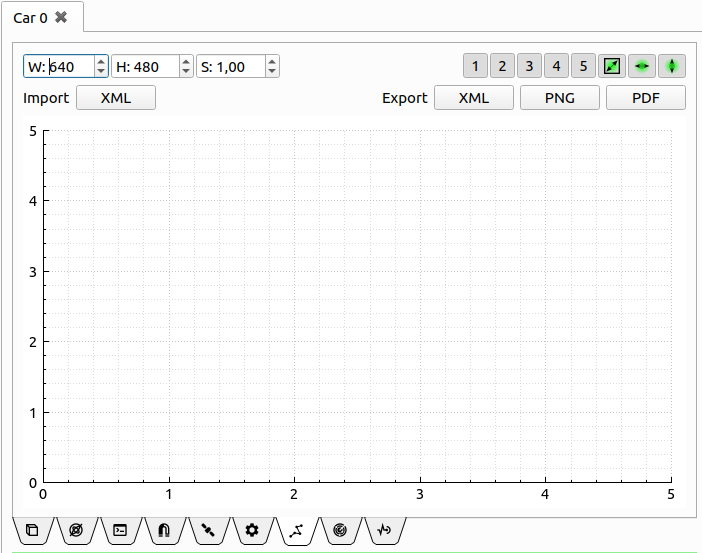
\includegraphics[width=\textwidth]{./screens/Car_experiment_plot.png}
\end{minipage}
\begin{minipage}{0.5\textwidth} %% Text Car Experiment
  \todo{text}
\end{minipage}
%% ------------------------------------------------------------

%% ------------------------------------------------------------
\begin{minipage}{0.5\textwidth} %% Text Car Radar
  \todo{text}
\end{minipage}
\begin{minipage}{0.5\textwidth}
  \noindent 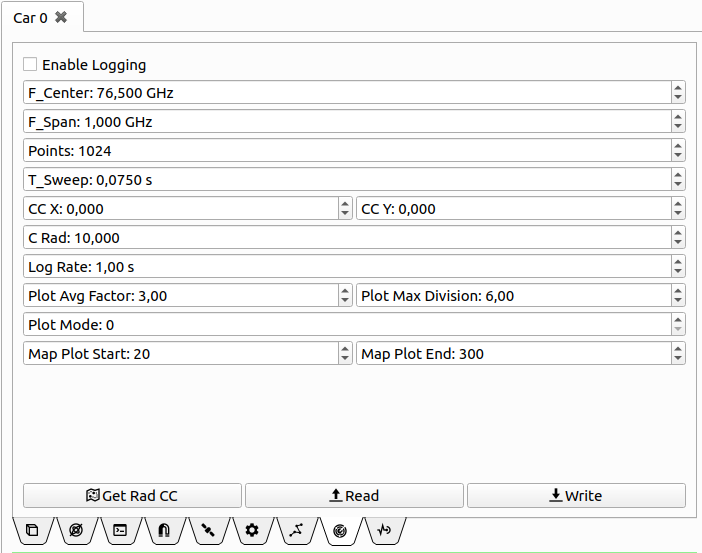
\includegraphics[width=\textwidth]{./screens/Car_radar.png}    
\end{minipage}
%% ------------------------------------------------------------


%% ------------------------------------------------------------
\begin{minipage}{0.5\textwidth}
  \noindent 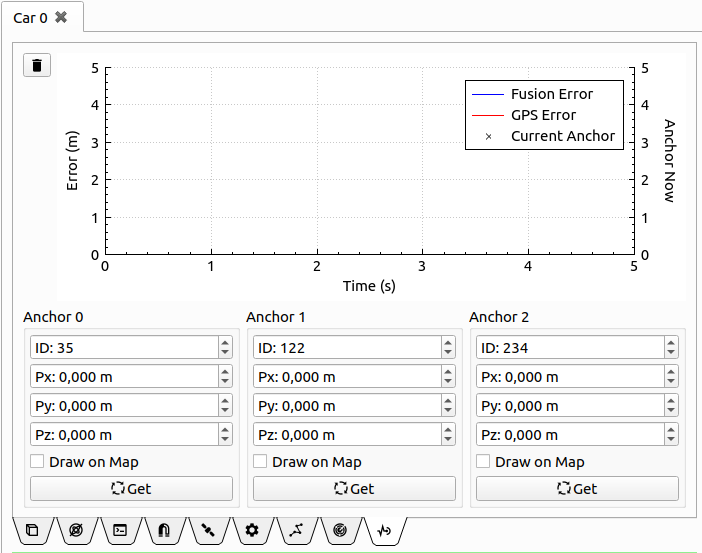
\includegraphics[width=\textwidth]{./screens/Car_UWB.png}
\end{minipage}
\begin{minipage}{0.5\textwidth} %% Text Car UWB
  \todo{text}
\end{minipage}
%% ------------------------------------------------------------


\subsection{Quadcopters}
\label{sec:quads}

%% ------------------------------------------------------------
\begin{minipage}{0.5\textwidth}
  \todo{text}
\end{minipage}
\begin{minipage}{0.5\textwidth}
  \noindent 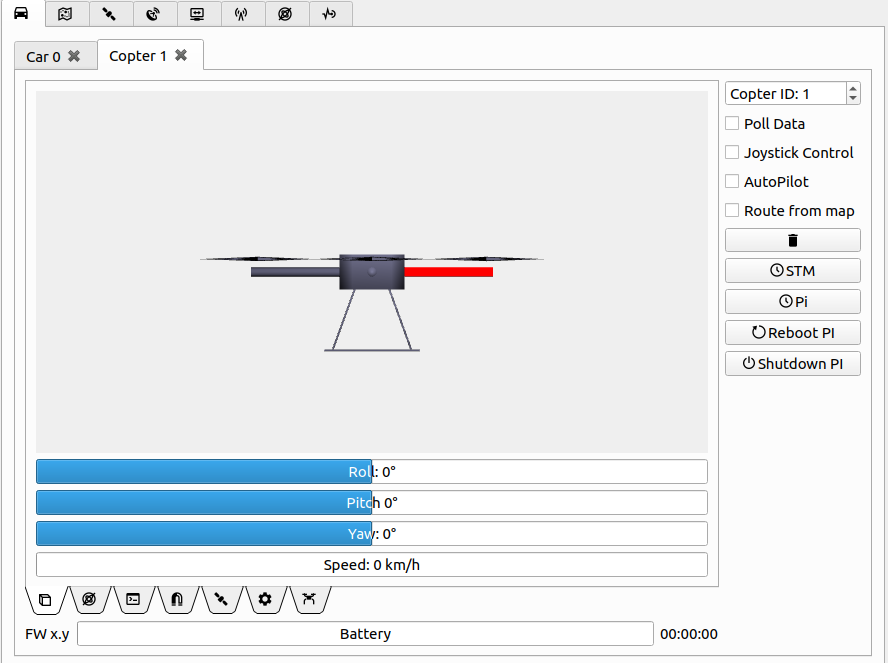
\includegraphics[width=\textwidth]{./screens/quad_orientation.png}
\end{minipage}
%% ------------------------------------------------------------


%% ------------------------------------------------------------
\begin{minipage}{0.5\textwidth}
  \noindent 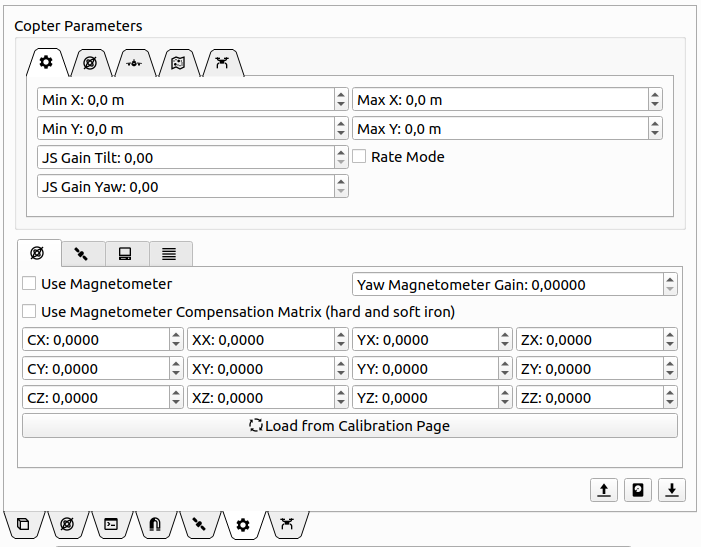
\includegraphics[width=\textwidth]{./screens/Quad_parameters.png}
\end{minipage}
\begin{minipage}{0.5\textwidth}
  \todo{text}
\end{minipage}
%% ------------------------------------------------------------

%% ------------------------------------------------------------
\begin{minipage}{0.5\textwidth}
  \todo{text}
\end{minipage}
\begin{minipage}{0.5\textwidth}
  \noindent 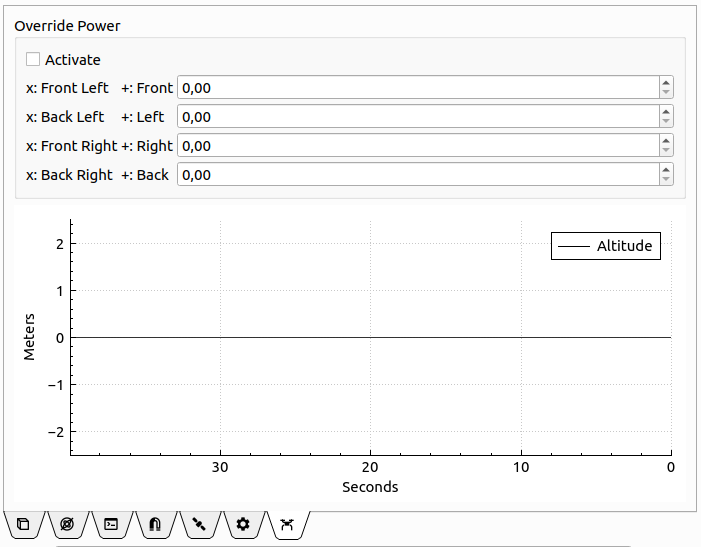
\includegraphics[width=\textwidth]{./screens/Quad_tests.png}
\end{minipage}
%% ------------------------------------------------------------


\todo{Write}

\subsection{Map}

\noindent 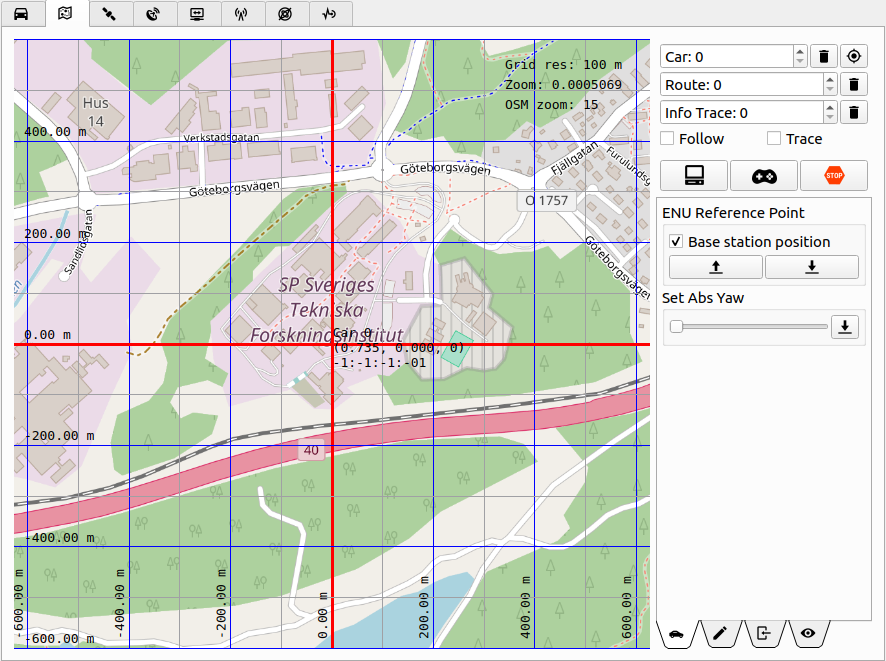
\includegraphics[width=\textwidth]{./screens/map_car_control.png}


%\begin{minipage}{0.25\textwidth}
\noindent 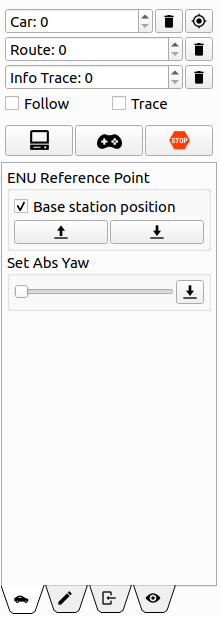
\includegraphics[width=0.25\textwidth,height=12cm]{./screens/map_car_control_panel.png}
%\end{minipage}
%\begin{minipage}{0.25\textwidth}
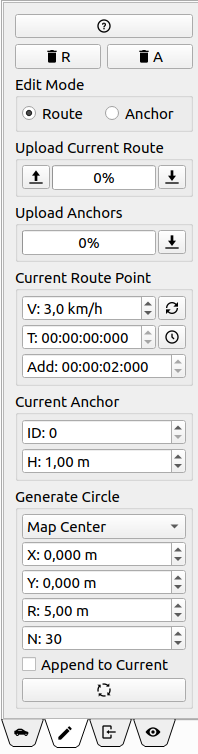
\includegraphics[width=0.25\textwidth,height=12cm]{./screens/map_edit_panel.png}
%\end{minipage}
%\begin{minipage}{0.25\textwidth}
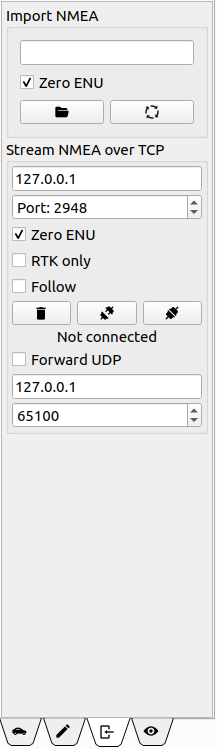
\includegraphics[width=0.25\textwidth,height=12cm]{./screens/map_import_panel.png}
%\end{minipage}
%\begin{minipage}{0.25\textwidth}
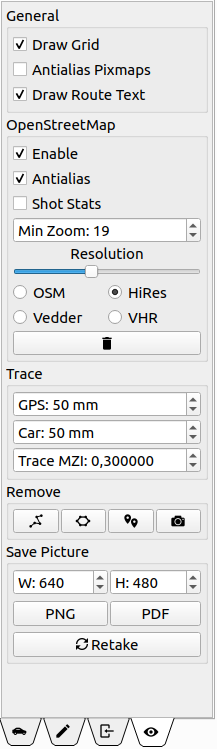
\includegraphics[width=0.25\textwidth,height=12cm]{./screens/map_view_panel.png}
%\end{minipage}


\subsubsection{Keyboard Shortcuts}
  
\begin{itemize} 
  \item {\bf CTRL + Right click:} Update route point or anchor settings
  \item {\bf Shift + Left click:} Add route point or anchor
  \item {\bf Shift + Left drag:} Move route point or anchor
  \item {\bf Shift + right click:} Delete route point or anchor
  \item {\bf CTRL + SHIFT + Left click:} Zero map ENU coordinates
\end{itemize} 

\subsection{RTCM Client}

\noindent 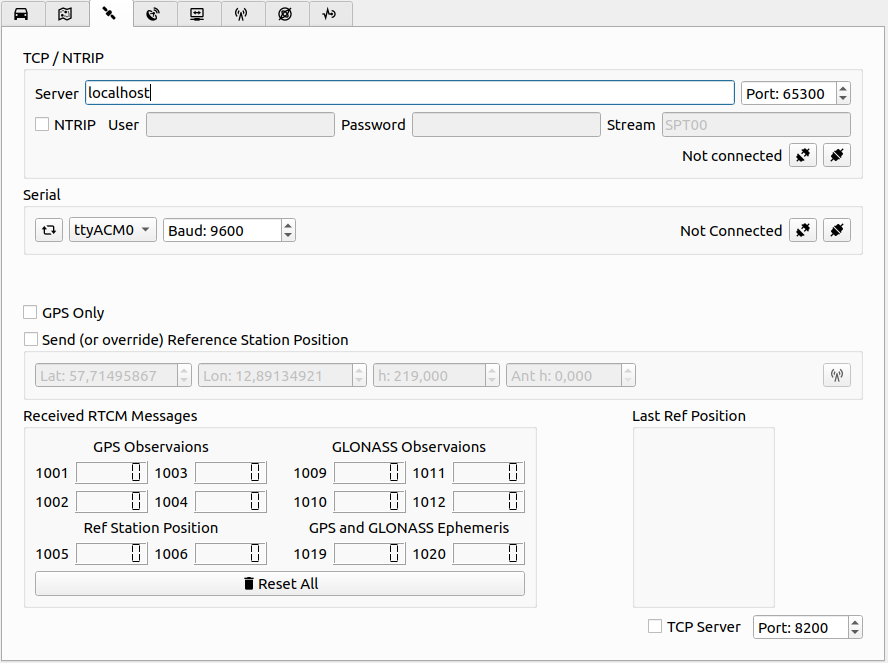
\includegraphics[width=\textwidth]{./screens/RTCM_client.png}

\todo{Write}

\subsection{Base Station}

\noindent 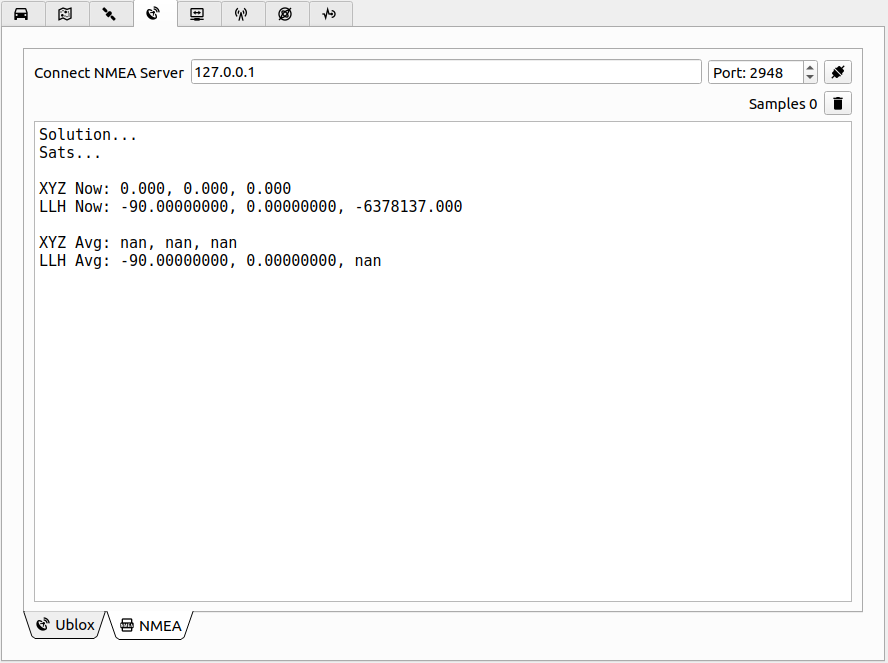
\includegraphics[width=\textwidth]{./screens/base_station_NMEA.png}

\noindent 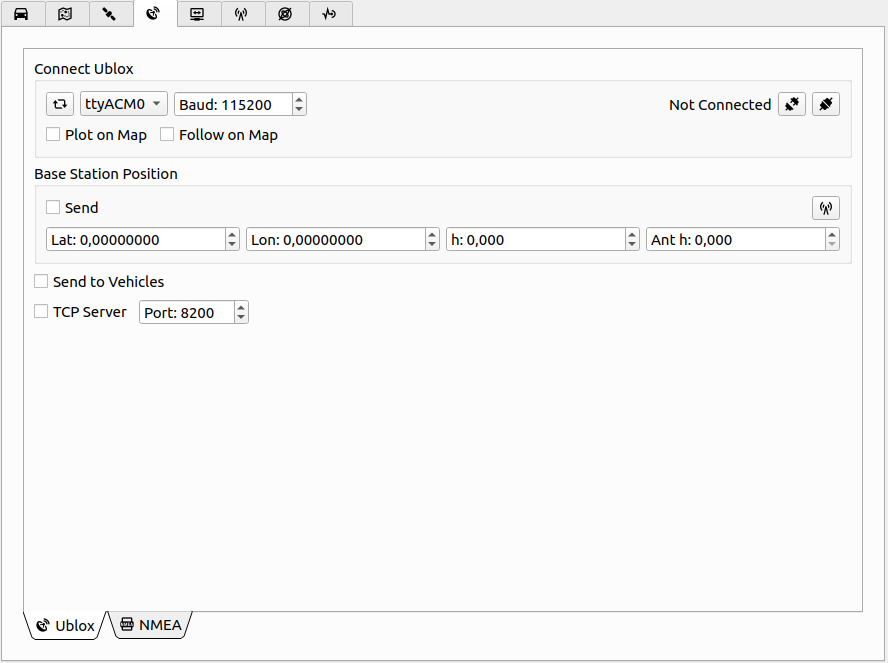
\includegraphics[width=\textwidth]{./screens/base_station_UBLOX.png}

\todo{Write}

\subsection{Network Interface}

\noindent 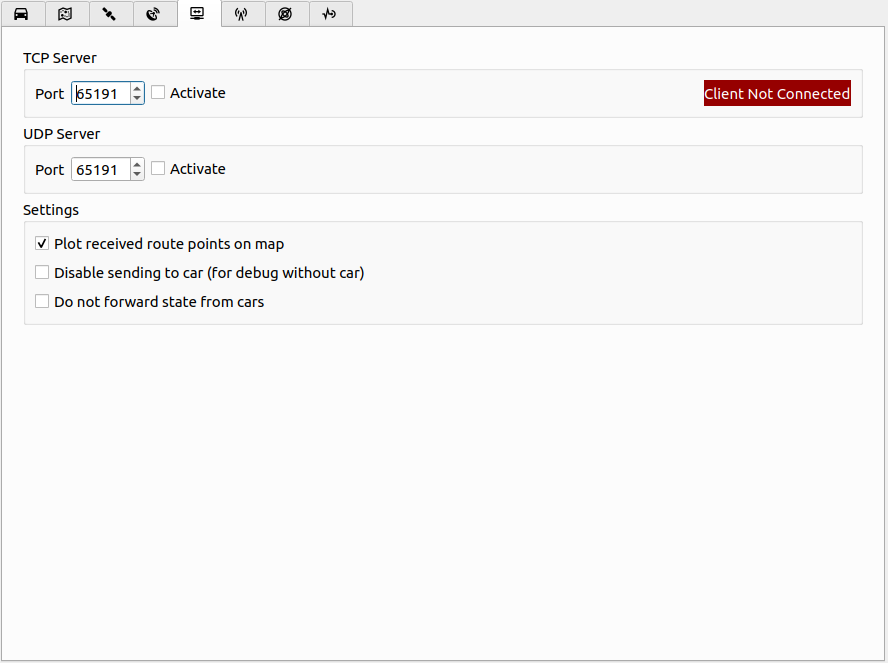
\includegraphics[width=\textwidth]{./screens/network_interface.png}

\todo{Write}

\subsection{Mote}

\noindent 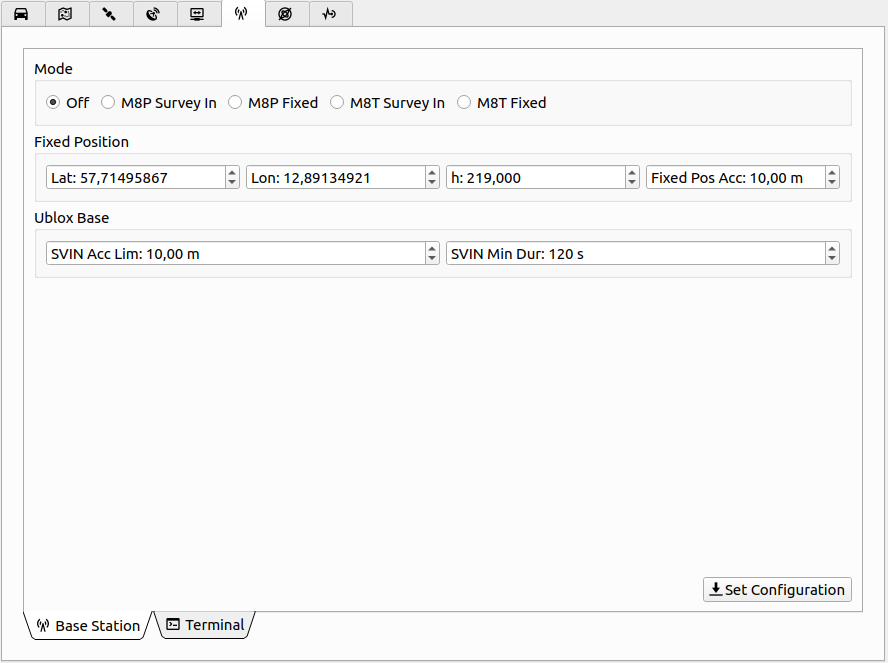
\includegraphics[width=\textwidth]{./screens/mote.png}

\todo{Write}

\subsection{NCom CLient}

\noindent 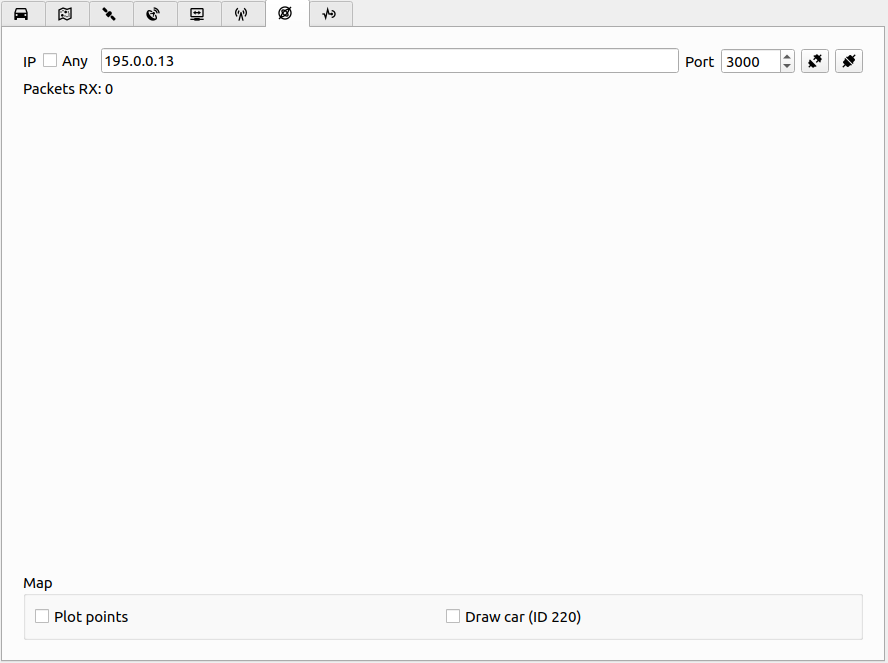
\includegraphics[width=\textwidth]{./screens/ncom_client.png}

\todo{Write}

\subsection{Logging and Analysis}

\noindent 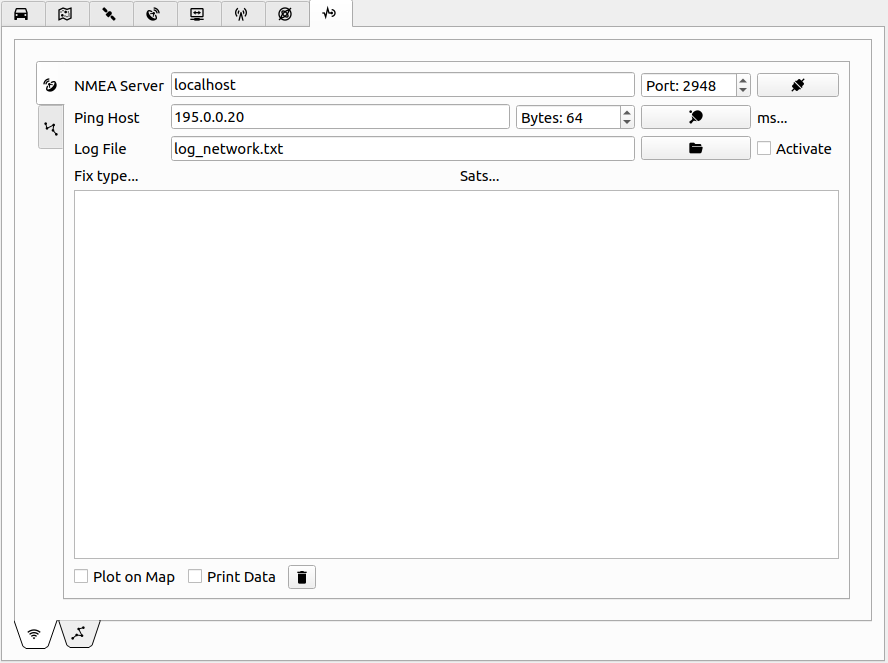
\includegraphics[width=\textwidth]{./screens/Log1.png}

\noindent 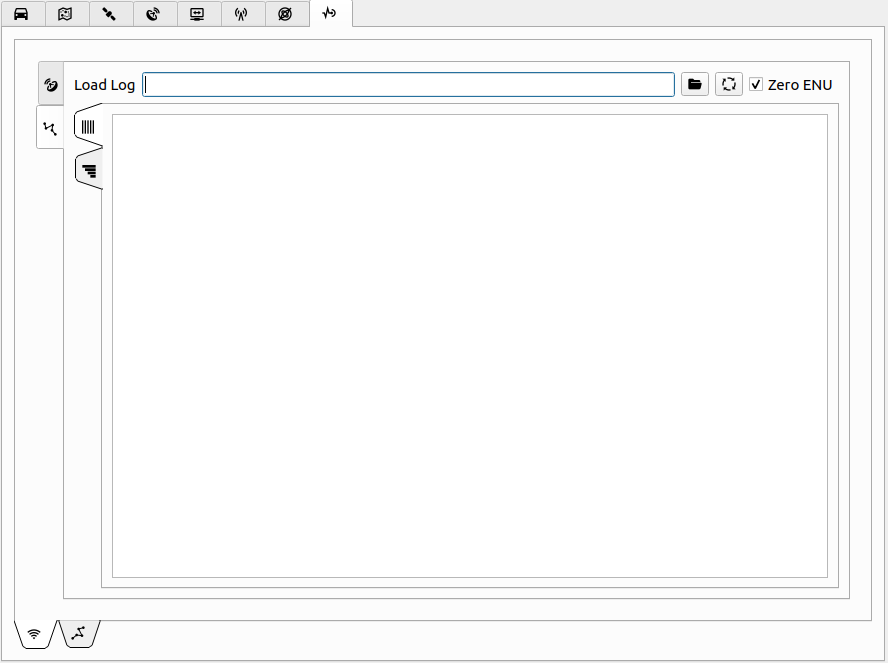
\includegraphics[width=\textwidth]{./screens/Log2.png}

\noindent 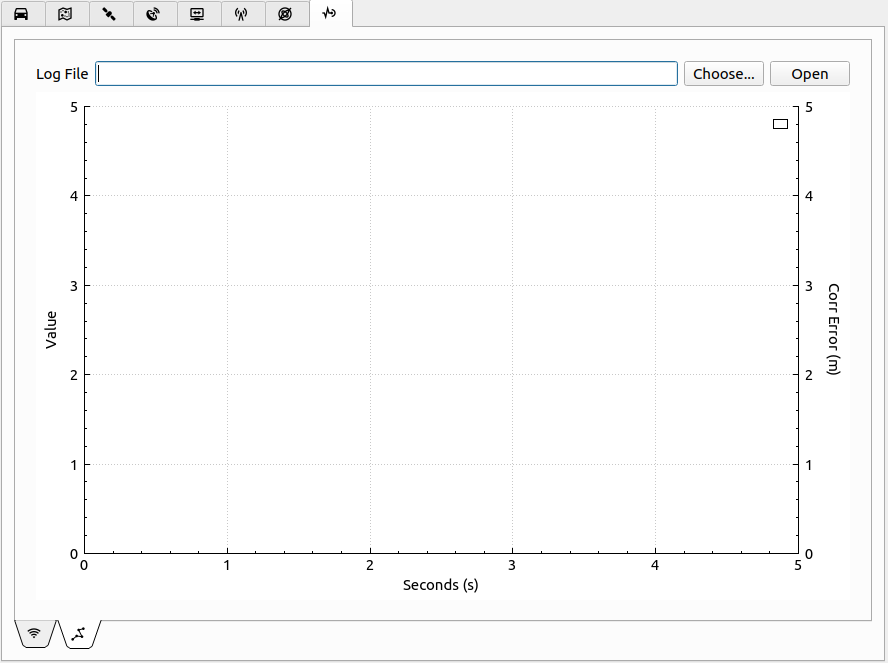
\includegraphics[width=\textwidth]{./screens/Log3.png}

\todo{Write}

\section{Example Setup: HIL Simulation Rig}

\todo{Write}

\section{Example Setup: Fully Operational System}

\todo{Write}

\section{Operation of the Full System}

\todo{ is it possible to describe how to do this in some tutorial fashion? }



\section{RControlStationComm Library}

\todo{Write}
\subsection{C++ library}

\begin{Verbatim}
class RCONTROLSTATIONCOMMSHARED_EXPORT RControlStationComm
{

public:
    RControlStationComm();
    ~RControlStationComm();
    bool connectTcp(QString host, int port);
    void disconnectTcp();
    void setDebugLevel(int level);
    bool hasError();
    char *lastError();
    bool getState(int car, CAR_STATE *state, int timeoutMs = 1000);
    bool getEnuRef(int car, bool fromMap, double *llh, int timeoutMs = 1000);
    bool setEnuRef(int car, double *llh, int timeoutMs = 1000);
    bool addRoutePoints(int car, ROUTE_POINT *route, int len,
                        bool replace = false, bool mapOnly = false,
                        int mapRoute = -1, int timeoutMs = 1000);
    bool clearRoute(int car, int mapRoute = -1, int timeoutMs = 1000);
    bool setAutopilotActive(int car, bool active, int timeoutMs = 1000);
    bool rcControl(int car, int mode, double value, double steering);
    bool getRoutePoints(int car, ROUTE_POINT *route, int *len,
                        int maxLen = 500, int mapRoute = -1, int timeoutMs = 1000);
    bool sendTerminalCmd(int car, char *cmd, char *reply, int timeoutMs = 1000);

private:
    struct ERROR_MSG {
        QString command;
        QString description;
    };

    QTcpSocket *mTcpSocket;
    int mDebugLevel;
    QByteArray mRxBuffer;
    QVector<QByteArray> mXmlBuffer;
    QVector<ERROR_MSG> mErrorMsgs;
    char mTextBuffer[10000];

    // CoreApplication
    QCoreApplication *mApp;
    int mAppArgc;
    char const *mAppArgv[2];

    void processData(const QByteArray &data);
    void sendData(const QByteArray &data);
    QByteArray waitForXml(int timeoutMs = 1000);
    bool waitForAck(QString cmd, int timeoutMs = 1000);
    bool isTcpConnected();
    QByteArray requestAnswer(int car, QString cmd, int timeoutMs = 1000);
    bool checkError(QString xml);

};
\end{Verbatim}

\todo{Explanation and example of use} 


\subsection{C library}

\begin{Verbatim}
bool rcsc_connectTcp(const char* host, int port);
void rcsc_disconnectTcp(void);
void rcsc_setDebugLevel(int level);
bool rcsc_hasError();
char *rcsc_lastError();
bool rcsc_getState(int car, CAR_STATE *state, int timeoutMs);
bool rcsc_getEnuRef(int car, bool fromMap, double *llh, int timeoutMs);
bool rcsc_setEnuRef(int car, double *llh, int timeoutMs);
bool rcsc_addRoutePoints(int car, ROUTE_POINT *route, int len,
                         bool replace, bool mapOnly,
                         int mapRoute, int timeoutMs);
bool rcsc_clearRoute(int car, int mapRoute, int timeoutMs);
bool rcsc_setAutopilotActive(int car, bool active, int timeoutMs);
bool rcsc_rcControl(int car, int mode, double value, double steering);
bool rcsc_getRoutePoints(int car, ROUTE_POINT *route, int *len,
                         int maxLen, int mapRoute, int timeoutMs);
bool rcsc_sendTerminalCmd(int car, char *cmd, char *reply, int timeoutMs);
\end{Verbatim} 


\todo{Explanation and example of use} 


\section{Networking and Connectivity Related Topics}

\todo{Figure out what this section should be called and what subsections it should have}

\subsection{Radios} 

\subsection{TCP, SSH and Tunnels}

\subsection{Correction data}


\newpage 
\section*{Changelog}

\begin{changeentry}{2018-X-Y}{Joel}
Initial version focusing on the RControlStation GUI. 
\end{changeentry}


%% \begin{figure}[]
%% \begin{minipage}{.42\textwidth}
%% \includegraphics[width=\textwidth]{./hls/hls_step5_prj_config4}
%% \end{minipage}
%% \begin{minipage}{.55\textwidth}
%% \includegraphics[width=\textwidth]{./hls/hls_step6_prj_device_select}
%% \end{minipage}
%% \caption{Solution configuration. Select the ``xc7z010clg225-1'' device.} 
%% \label{fig:hls5to6}
%% \end{figure}

%\thispagestyle{fancy}

% \begin{abstract}
% \end{abstract}


%% \let\oldbibliography\thebibliography
%% \renewcommand{\thebibliography}[1]{%
%%   \oldbibliography{#1}%
%%   \setlength{\itemsep}{1pt}%
%% }

%% {\small
%% % \vspace{-40mm}
%% %\bibliographystyle{abbrvnat}
%% %\bibliographystyle{plain}
%% \bibliographystyle{abbrv}
%% \bibliography{../VR2016/refs}
%% % \bibliography{./refs}
%% }

\end{document}
